\pdfobjcompresslevel=0
\pdfminorversion=9
\documentclass[aspectratio=169]{beamer}

\usepackage[utf8]{inputenc}
\usetheme{Oxygen}
\setbeamersize{text margin left=3mm,text margin right=3mm}

\usepackage{graphicx}
\usepackage{hyperref}
\usepackage{textpos}
\usepackage{fancybox}
\usepackage{rotating}
\usepackage{subfigure}
\usepackage{multicol}
\usepackage{multirow}
\usepackage{array}
\usepackage{booktabs}
\usepackage{tabularx}
\usepackage{tabularray}
\usepackage{colortbl}
\usepackage{arydshln}
\usepackage{breakcites}
\usepackage{ragged2e}
\usepackage{adjustbox}
\usepackage{etoolbox}
\usepackage{xifthen}
\usepackage{xstring}
\usepackage[nopar]{lipsum}

\usepackage{amsmath,amssymb,amsfonts,amsbsy,dsfont}
\usepackage{mathrsfs}
\usepackage{amsthm}
\usepackage{bm}

\usepackage[table]{xcolor}
\usepackage{pifont}

\usepackage{tikz}
\usepackage{pgfplots}
\usepackage{pgfplotstable}
\pgfplotsset{compat=1.18}

\usetikzlibrary{
    calc,
    intersections,
    backgrounds,
    arrows.meta,
    positioning,
    shapes,
    shadows,
    shapes.geometric,
    fit,
    angles,
    quotes,
    decorations.pathreplacing,
    mindmap,
    bending
}

\usepgfplotslibrary{statistics,fillbetween}

% PGF layers required by figures/Giga.tex
\pgfdeclarelayer{background}
\pgfdeclarelayer{foreground}
\pgfsetlayers{background,main,foreground}

% Citations smaller
\let\oldcite\cite
\renewcommand{\cite}[1]{{\tiny\oldcite{#1}}}

% Unicode minus
\DeclareUnicodeCharacter{2212}{-}

% Basic math commands
\providecommand{\mat}[1]{{\bm{#1}}}
\providecommand{\ve}[1]{{\bm{#1}}}
\newcommand{\x}{\negthinspace\times\negthinspace}
\newcommand{\Real}{\mathbb{R}}
\newcommand{\N}{\mathbb{N}}
\newcommand{\unos}{\ve{1}}
% \providecommand{\kernel}[2]{\kappa\left(#1,#2\right)}

% Glossary fallback for figures
\providecommand{\gls}[1]{\MakeUppercase{#1}}
\providecommand{\glspl}[1]{\MakeUppercase{#1}s}

% Figure draft mode
\newif\iffigdraft
\figdraftfalse

\newcommand{\rasterpdffile}[3][]{%
  \def\dpi{#1}%
  \ifthenelse{\isempty{#1}}{\iffigdraft\def\dpi{150}\else\def\dpi{300}\fi}{}%
  \StrBefore{#2}{.pdf}[\base]%
  \IfFileExists{\base.ras@\dpi.png}{}{%
    \immediate\write18{gs -q -dSAFER -dBATCH -dNOPAUSE -sDEVICE=pngalpha -r\dpi
      -dFirstPage=1 -dLastPage=1 -o "\base.ras@\dpi.png" "#2"}%
  }%
  \includegraphics[width=#3]{\base.ras@\dpi.png}%
}

% Custom itemize
\newif\ifcomment
\newcommand{\Com}{\par\footnotesize\itshape\commenttrue}

\newenvironment{Itemize}
 {%
  \edef\Itemizecurrent{\the\font}%
  \itemize
  \preto{\item}{\ifcomment\par\Itemizecurrent\fi}%
 }{%
  \enditemize
 }

% Row colors and marks
\definecolor{completed}{RGB}{232,246,239}
\definecolor{writing}{RGB}{255,237,213}
\newcommand{\cmark}{\checkmark}
\newcommand{\wmark}{\textbf{W}}

% Colors for electrode figures
\DeclareRobustCommand{\legend}[1]{%
  \textcolor{#1}{\rule{1ex}{2ex}}%
}

\definecolor{frontal_left}{RGB}{255,237,111}
\definecolor{frontal}{RGB}{141,211,199}
\definecolor{frontal_right}{RGB}{255,255,179}
\definecolor{central_left}{RGB}{204,235,197}
\definecolor{central_right}{RGB}{188,128,189}
\definecolor{centro_parietal_left}{RGB}{190,186,218}
\definecolor{centro_parietal_right}{RGB}{128,177,211}
\definecolor{parietal_left}{RGB}{217,217,217}
\definecolor{parietal_right}{RGB}{253,141,60}
\definecolor{posterior}{RGB}{179,222,105}

\definecolor{Orange}{HTML}{FDB463}
\colorlet{posterior_right}{Orange}

\definecolor{GrayL}{HTML}{D8D8D9}
\colorlet{posterior_left}{GrayL}

\definecolor{UpperGreen}{HTML}{8DD3C8}
\definecolor{LowerYellow}{HTML}{FEFFB3}
\definecolor{BlueRightSide}{HTML}{80B0D3}
\definecolor{PurpleLeftSide}{HTML}{BD80BD}
\definecolor{Purple}{HTML}{BFBADA}
\definecolor{GrayC}{HTML}{D8D8D9}
\definecolor{GreenC}{HTML}{CDEBC4}
\definecolor{GreenD}{HTML}{B2DF6A}
\definecolor{YellowC}{HTML}{FEEC6F}
\definecolor{ElecBG}{HTML}{CFE7E2}
\definecolor{mypink1}{rgb}{0.858,0.188,0.478}

% Separation parameter used in montage figures
\def\sep{0.27}

% Electrode style
\tikzset{
  electrode/.style={
    draw,
    line width=0.5pt,
    circle,
    inner sep=1pt,
    minimum size=6mm,
    fill=ElecBG,
    font=\scriptsize
  }
}
\definecolor{paperblue}{RGB}{220,235,255}
\definecolor{frameblue}{RGB}{25,74,155}
%%%%%%%%%%%%%%%%%%%%%%%%%%%%%%%%%%%%%%%%%%%%%%%%%%%%%%
%%%%%%%


\title[Connectivity-Based Deep Learning for EEG Decoding in Brain–Computer Interfaces| Y.A Gomez Rivera] {Connectivity-Based Deep Learning for EEG Decoding in Brain–Computer Interfaces}

\author[A. Gomez Rivera] {}
\institute{\small{Yessica Alejandra Gomez Rivera}\\
{\small\textbf{ Advisor:} Prof. Andrés Marino Álvarez-Meza}\\
{\small \textbf{Co-Advisor:} Prof. David Cárdenas Peña \\ 
 }
 
 
 
\includegraphics[width=0.12\textwidth]{EscudoUN.png}\\
 
 \scriptsize{
Universidad Nacional de Colombia \\ Signal Processing and Recognition Group - SPRG \\ Manizales, Colombia 

\vspace{-0.3cm}
}}
\date[]{\scriptsize{\today}}

\setbeamercovered{dynamic}
\setbeamertemplate{navigation symbols}{}

%----------------------------------------------------
% Forzar eliminación de cualquier logo insertado por el tema
\logo{}
\setbeamertemplate{logo}{}
\renewcommand{\insertlogo}{}
%---------------------------------------------------
\begin{document}

{\setbeamertemplate{headline}{}
\setbeamertemplate{footline}{}
\begin{frame}{}
\vspace{-0.7cm}
    \titlepage 
\end{frame}
}


%----------------------------------------------------
\begin{frame}{Outline} 
\tableofcontents 
\end{frame}

%%%%%%%%%%%%%%%%%%%%%%%%%%%%%%%%%%%%%%%%%
\section[Motivation]{Motivation}
%--------------------------------------------
\begin{frame}{Brain–Computer Interfaces (BCIs)}
\centering Establish a direct connection between the human brain and a computer\cite{padfield2019eeg}

\begin{figure}
    \centering
    \includegraphics[width=0.92\linewidth]{figures/BCI.pdf}
    \label{fig:Motivation1}
\end{figure}

\textcolor{frameblue}{BCIs also have a growing economic impact, with the global market \\ 
expanding steadily (Compound Annual Growth Rate, CAGR: 10.29\%)~\cite{mordor2025bci}}
\end{frame}

%--------------------------------------------
\begin{frame}{Applications of BCI Systems}

\centering
BCI systems translate brain activity into commands or feedback for diverse applications

\begin{columns}[t,onlytextwidth]

    %----------------------------------------
    \begin{column}{0.47\textwidth}
    \raggedright
    \footnotesize
    
    \textbf{Clinical applications}
    \begin{itemize}\setlength\itemsep{0.18cm}
        \item Assistive communication {\scriptsize \cite{edelman2025noninvasive}}
        \item Neuroprosthetic control {\scriptsize \cite{he2024bci}}
        \item Neurorehabilitation {\scriptsize \cite{edelman2025noninvasive}}
    \end{itemize}

    \vspace{0.05cm}

    \textbf{Non-clinical applications}
    \begin{itemize}\setlength\itemsep{0.18cm}
        \item Video game control {\scriptsize \cite{alvarez2024gaming}}
        \item Human--computer interaction {\scriptsize \cite{ghosh2024multimodal}}
        \item BCI-based cognitive training \\  \cite{rashid2024cognitive}
    \end{itemize}

    \end{column}

    %----------------------------------------
    \begin{column}{0.51\textwidth}
    \vspace{-2mm}
    \begin{figure}
        \centering
        \includegraphics[width=0.65\linewidth]{figures/APPLICATIONS.pdf}
    \end{figure}
    \end{column}

\end{columns}
\textcolor{frameblue}{BCIs enable direct interaction between neural activity and external devices or \\ feedback systems \cite{pang2024advancements}}

\end{frame}
%--------------------------------------------

\begin{frame}{Types of BCI Sensor Setups}
\centering{Invasive (ECoG), and non-invasive (MEG, fMRI, fNIRS, EEG)\cite{ghosh2024multimodal}}
\begin{figure}
    \centering
    \includegraphics[width=0.65\linewidth]{figures/Motivation 2.pdf}
    \label{fig:Motivation2}

\centering \textcolor{frameblue}{This doctoral research proposal focuses on EEG due to its practical balance between accessibility, portability, and temporal resolution \cite{edelman2025noninvasive}}
\end{figure}
\end{frame}

%--------------------------------------------

\begin{frame}{Primary EEG application paradigms addressed in this research}
\centering{The cognitive activity of imagining a movement without actually performing it \cite{mustile2024neural}}

\begin{figure}
    \centering
    \includegraphics[width=0.5\linewidth]{figures/MI-TDHA.pdf}
    \label{fig:MI-TDHA}
\end{figure}
\centering\textcolor{frameblue}{EEG recorded during attention-demanding cognitive tasks is analyzed to support clinical decision-making for Attention-Deficit/Hyperactivity Disorder (ADHD) \cite{li2025adhd}}
\end{frame}

%----------------------------------------------------
%AQUI
%--------------------------------------------
\begin{frame}{Types of Brain Connectivity}
% \scriptsize

\begin{columns}[t,onlytextwidth]

    %-------------------------------------------------
    \column{0.32\textwidth}
    \centering
    {\small \textbf{Structural Connectivity}}\\[-0.02cm]
    {\scriptsize \cite{sporns2007brain, siviero2023functional}}\\[0.15cm]

    \begin{itemize}\scriptsize
        \item Describes physical anatomical links between brain regions
        \item Usually estimated using diffusion imaging, e.g., DTI/dMRI
    \end{itemize}

    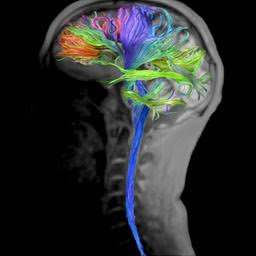
\includegraphics[width=0.58\linewidth]{figures/Cdqdee8W8AAIwJF.jpg}

    {\scriptsize \textit{What is physically connected?}}

    %-------------------------------------------------
    \column{0.32\textwidth}
    \centering
    {\small \textbf{Functional Connectivity}}\\[-0.02cm]
    {\scriptsize \cite{sporns2007brain, fornito2024connectomics}}\\[0.15cm]

    \begin{itemize}\scriptsize
        \item Measures statistical dependence between brain signals
        \item Captures synchronization or co-activation patterns
    \end{itemize}

    \includegraphics[width=0.58\linewidth]{figures/Fuctional.pdf}

    {\scriptsize \textit{Which regions co-vary over time?}}

    %-------------------------------------------------
    \column{0.32\textwidth}
    \centering
    {\small \textbf{Effective Connectivity}}\\[-0.02cm]
    {\scriptsize \cite{granger1969investigating, ma2024dtfgraph}}\\[0.15cm]

    \begin{itemize}\scriptsize
        \item Estimates directed or predictive interactions in brain regions
        \item Describes information flow among neural signals
    \end{itemize}

\includegraphics[width=0.58\linewidth]{figures/Efective.pdf}

    {\scriptsize \textit{Who provides information to whom?}}

\end{columns}
\begin{center}
\textcolor{frameblue}{Functional and effective connectivity allow EEG-based analysis to move from isolated channel \\ activity to inter-channel interactions \cite{ma2024dtfgraph}}
\end{center}

\end{frame}
%--------------------------------------------
\begin{frame}{Causality and Effective Connectivity in EEG}

\scriptsize
\setlength{\abovedisplayskip}{2pt}
\setlength{\belowdisplayskip}{2pt}
\setlength{\jot}{1pt}

\begin{columns}[T,totalwidth=\textwidth]

%==================================================
% LEFT COLUMN
%==================================================
\begin{column}{0.48\textwidth}

\textbf{Physical model: sources $\rightarrow$ sensors}

\vspace{0.08cm}

\[
\mathbf{s}_t = F(\mathbf{s}_{t-1},\mathbf{u}_t,\theta)+\mathbf{w}_t,
\qquad
\mathbf{x}_t = \mathbf{L}\mathbf{s}_t+\boldsymbol{\eta}_t
\]

\vspace{0.02cm}

{\tiny
$\mathbf{s}_t$: latent neural sources; $\mathbf{x}_t$: scalp EEG;
$\mathbf{L}$: source mixing / lead-field; $\boldsymbol{\eta}_t$: noise
}

\vspace{0.14cm}

\textbf{Use in neuroscience}

\vspace{0.05cm}

\begin{itemize}\itemsep2pt
    \item \textbf{Effective connectivity} describes directed influence among
    neural systems \cite{friston1994functional}
    
    \item In neuroscience, \textbf{causal connectivity} is often used in this
    operational sense: directed statistical influence, not strict physical
    causality \cite{seth2015granger}
    
    \item In scalp EEG, interpretation must be cautious because sensors mix
    multiple sources through volume conduction \cite{haufe2013critical}
\end{itemize}

\end{column}

%==================================================
% RIGHT COLUMN
%==================================================
\begin{column}{0.50\textwidth}

\textbf{Mathematical model: Granger causality}

\vspace{0.05cm}

\[
\begin{aligned}
Y_t &= \sum_{k=1}^{p} a_{yy,k}Y_{t-k}+\varepsilon_t,\\
Y_t &= \sum_{k=1}^{p} a_{yy,k}Y_{t-k}
     +\sum_{k=1}^{p} a_{yx,k}X_{t-k}+\varepsilon'_t
\end{aligned}
\]

\vspace{-0.05cm}

\[
GC_{X\rightarrow Y}
=
\ln
\left(
\frac{\mathrm{var}(\varepsilon_t)}
{\mathrm{var}(\varepsilon'_t)}
\right)
\]

\vspace{0.02cm}

{\tiny
$X$ Granger-causes $Y$ if the past of $X$ improves the prediction of $Y$
beyond the past of $Y$ itself \cite{granger1969investigating,seth2015granger}.
}

\vspace{0.12cm}

\textbf{Main assumptions}

\vspace{0.04cm}

{\tiny
Temporal precedence, adequate sampling, suitable model order, stationarity
or proper treatment of nonstationarity, and conditioning on relevant variables.
If these assumptions are violated, Granger causality may produce statistically
significant but physiologically implausible directed links
\cite{stokes2017study}
}

\end{column}

\end{columns}

\vspace{0.06cm}

{\centering
\color{frameblue}\footnotesize
In this proposal, causal connectivity is interpreted as directed effective
connectivity in the predictive Granger sense, not as proof of strict physical
causality
\par}

\end{frame}
%--------------------------------------------
\begin{frame}{From Handcrafted Features to Deep Learning}

\centering
\includegraphics[width=0.65\linewidth]{figures/ML VS DL.pdf}

\centering\textcolor{frameblue}{Machine learning and deep learning techniques have reduced the reliance on handcrafted features, enabling end-to-end learning from minimally processed signals {\tiny{\cite{lee2025review}}}}
\end{frame}
%--------------------------------------------

\begin{frame}{Research Groups Supporting this Doctoral Research}

\begin{figure}
    \centering
    \includegraphics[width=0.52\linewidth]{figures/grupos.pdf}
    \label{fig:grupos}
\end{figure}

\centering\textcolor{frameblue}{They integrate signal processing, machine learning, EEG analysis, and computer vision to develop robust methodologies for assessment, monitoring, and cognitive decoding}
\end{frame}
%--------------------------------------------

\begin{frame}{ACEMATE Program}
\begin{figure}
    \centering
    \includegraphics[width=0.95\linewidth]{figures/Acemate.pdf}
    \label{fig:acemate}
\end{figure}

\begin{center}
\centering\textcolor{frameblue}{EEG connectivity-based deep learning for objective and interpretable neurocognitive assessment}
\end{center}

\end{frame}

% %--------------------------------------------

\section{Problem Statement}
%--------------------------------------------
\begin{frame}{Issue \#1: Noisy data and low spatial resolution}

\begin{figure}
    \centering
    \includegraphics[width=0.73\linewidth]{figures/Problem 1.pdf}
    \label{fig:problem1}
\end{figure}

\centering\textcolor{frameblue}{
EEG spatial specificity is limited by volume conduction, source mixing, and artifacts 
{\scriptsize \cite{nagy2024spatial}}
}

\end{frame}
%--------------------------------------------

\begin{frame}{Issue \#2: {Nonlinear and Nonstationary EEG Channel dependencies}}

\begin{figure}
    \centering
    \includegraphics[width=0.68\linewidth]{figures/Problem 2.pdf}
    \label{fig:problem2}
\end{figure}

\centering\textcolor{frameblue}{
Linear or symmetric connectivity measures are limited in capturing EEG's dynamic, nonlinear, 
\\ and directed interactions \cite{redondo2025spectral}
}

\end{frame}

%--------------------------------------------
\begin{frame}{Issue \#3: High inter- and intra-subject variability}
\begin{figure}
    \centering
    \includegraphics[width=0.6\linewidth]{figures/Problem 3.pdf}
    \label{fig:problem3}

\centering\textcolor{frameblue}{Inter- and intra-subject variability in EEG-based bci systems leading to overfitting and limited subject-independent generalization \cite{wang2024dmmr}}
\end{figure}
\end{frame}
%--------------------------------------------

\begin{frame}{Issue \#4: The Interpretability-Expressiveness Trade-off}

\centering
\includegraphics[width=0.55\linewidth]{figures/problem4.pdf}

\vspace{0.15cm}

{\centering
\textcolor{frameblue}{
Existing uninterpretable black-box deep learning models are untrustworthy and lack accountability in real-world applications, leading to a lack of trust \\ and hindering clinical adoption {\tiny\cite{barnett2024improving}}
}
\par}

\end{frame}
%--------------------------------------------

%--------------------------------------------
\begin{frame}{Research Question}

\begin{itemize}
\justifying
    \item How can an \textbf{interpretable deep learning framework} be designed for 
    \textbf{EEG-based BCI systems} to model \textbf{nonlinear, non-stationary, and directed brain connectivity}, 
    improve \textbf{generalization across subjects and sessions}, mitigate the effects of 
    \textbf{noise}, and address the \textbf{limited spatial resolution}?
\end{itemize}
\end{frame}
%--------------------------------------------

\section[Literature Overview]{Literature Overview}

% \subsection{EEG Decoding Models: Classical and End-to-End Deep Learning}

\begin{frame}{Classical EEG-based Models}
\centering

% --- Ajustes compactos ---
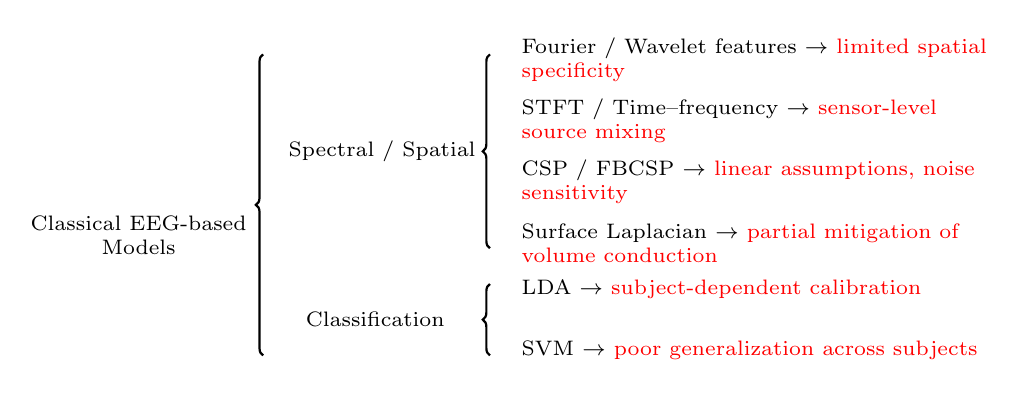
\begin{tikzpicture}[
  x=\linewidth, y=1.0cm, line width=0.8pt,
  font=\scriptsize,
  scale=1.08, every node/.style={transform shape} % <- reduce TODO (incluye texto)
]

% ===== spacing =====
\def\labelpad{0.012}
\def\topbot{0.06}
\def\dy{0.72}          
\def\yA{0.9}           
\def\gapBlocks{0.75}  
\def\amp{2.6pt}        

\pgfmathsetmacro{\yB}{\yA - (2 + \gapBlocks)*\dy}

% ===== styles =====
\tikzset{
  brace/.style={
    draw=none,
    postaction={draw,decorate,decoration={brace,mirror,raise=0pt,amplitude=\amp}}
  },
  lab/.style={anchor=east,fill=white,inner sep=1pt,align=center},
  glab/.style={anchor=east,fill=white,inner sep=1pt},
  item/.style={anchor=west,text width=0.46\linewidth} % <- antes 0.50 (más compacto)
}

% ===== column positions (un poco más a la izquierda) =====
\pgfmathsetmacro{\xMain}{0.28}
\pgfmathsetmacro{\xInner}{0.50}
\pgfmathsetmacro{\xText}{0.52}

% ===== labels =====
\def\Main{Classical EEG-based\\Models}
\def\A{Spectral / Spatial}
\def\B{Classification}

% ===== items =====
\def\Aone{Fourier / Wavelet features $\rightarrow$ \textcolor{red}{limited spatial specificity}}
\def\Atwo{STFT / Time--frequency $\rightarrow$ \textcolor{red}{sensor-level source mixing}}
\def\Athree{CSP / FBCSP $\rightarrow$ \textcolor{red}{linear assumptions, noise sensitivity}}
\def\Afour{Surface Laplacian $\rightarrow$ \textcolor{red}{partial mitigation of volume conduction}}
\def\Bone{LDA $\rightarrow$ \textcolor{red}{subject-dependent calibration}}
\def\Btwo{SVM $\rightarrow$ \textcolor{red}{poor generalization across subjects}}

% ===== main brace =====
\draw[brace] (\xMain,\yA+1.5*\dy+\topbot) -- (\xMain,\yB-0.5*\dy-\topbot);
\node[lab] at (\xMain-\labelpad, {(\yA+\yB)/2}) {\Main};

% ===== group braces =====
\draw[brace] (\xInner,\yA+1.5*\dy+\topbot) -- (\xInner,\yA-1.5*\dy-\topbot);
\draw[brace] (\xInner,\yB+0.5*\dy+\topbot) -- (\xInner,\yB-0.5*\dy-\topbot);

% ===== group labels =====
\node[glab] at (\xInner-0.01,\yA) {\A};
\node[glab] at (\xInner-0.04,\yB) {\B};

% ===== items =====
\node[item] at (\xText,\yA+1.5*\dy) {\Aone};
\node[item] at (\xText,\yA+0.5*\dy) {\Atwo};
\node[item] at (\xText,\yA-0.5*\dy) {\Athree};
\node[item] at (\xText,\yA-1.5*\dy) {\Afour};

\node[item] at (\xText,\yB+0.5*\dy) {\Bone};
\node[item] at (\xText,\yB-0.5*\dy) {\Btwo};

\end{tikzpicture}

\vspace{0.4em} 


\textbf{\scriptsize Relevant references:\cite{singh2021comprehensive,wang2019eeg,pan2025enhancing,alim2023signals_anovapca_svm}}

\vspace{1.0em} 

\begin{center}
    \centering\textcolor{frameblue}{
    Classical sensor-level EEG methods are affected by source mixing, volume conduction, noise, 
     and inter-subject variability, reducing spatial specificity and  cross-subject generalization 
\cite{zhong2025eegdg}
} 
\end{center}
\end{frame}

%--------------------------------------------   

\begin{frame}{End-to-End Deep Learning Models for EEG-based BCI}
\centering

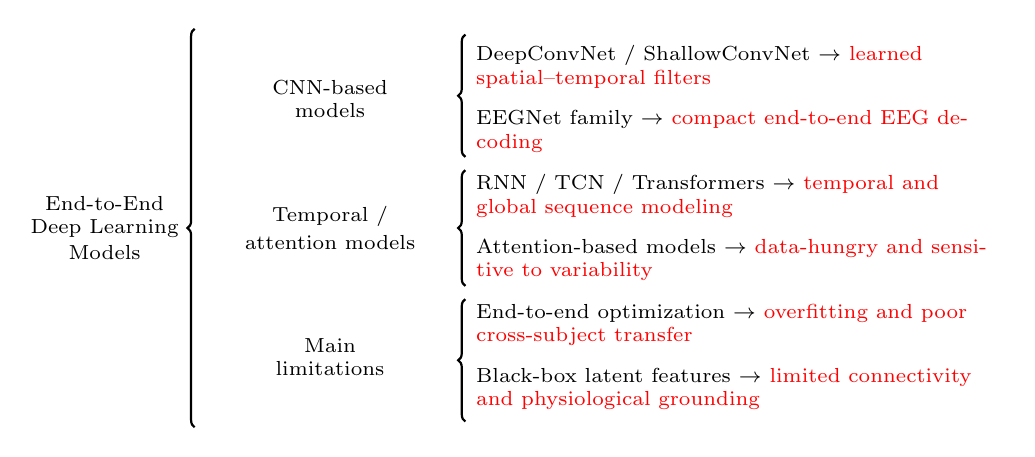
\begin{tikzpicture}[
  x=\linewidth, y=1.0cm, line width=0.8pt,
  font=\scriptsize,
  scale=1.05, every node/.style={transform shape}
]

% ===== spacing =====
\def\labelpad{0.012}
\def\topbotMain{0.07}
\def\topbotInner{0.00}
\def\dy{0.78}
\def\yT{2.05}
\def\amp{2.6pt}
\def\vgap{0.08}

% ===== styles =====
\tikzset{
  brace/.style={
    draw=none,
    postaction={draw,decorate,decoration={brace,mirror,raise=0pt,amplitude=\amp}}
  },
  lab/.style={anchor=east,fill=white,inner sep=1pt,align=center},
  glab/.style={anchor=center,fill=white,inner sep=1pt,align=center},
  item/.style={anchor=west,text width=0.52\linewidth}
}

% ===== column positions =====
\pgfmathsetmacro{\xMain}{0.26}
\pgfmathsetmacro{\xInner}{0.53}
\pgfmathsetmacro{\xText}{0.53}
\pgfmathsetmacro{\xMid}{(\xMain+\xInner)/2}

% ===== labels =====
\def\Main{\shortstack{End-to-End\\Deep Learning\\Models}}

\def\GOne{\shortstack{CNN-based\\models}}
\def\GTwo{\shortstack{Temporal /\\attention models}}
\def\GThree{\shortstack{Main\\limitations}}

% ===== items =====
\def\Ione{DeepConvNet / ShallowConvNet $\rightarrow$ \textcolor{red}{learned spatial--temporal filters}}
\def\Itwo{EEGNet family $\rightarrow$ \textcolor{red}{compact end-to-end EEG decoding}}

\def\Ithree{RNN / TCN / Transformers $\rightarrow$ \textcolor{red}{temporal and global sequence modeling}}
\def\Ifour{Attention-based models $\rightarrow$ \textcolor{red}{data-hungry and sensitive to variability}}

\def\Ifive{End-to-end optimization $\rightarrow$ \textcolor{red}{overfitting and poor cross-subject transfer}}
\def\Isix{Black-box latent features $\rightarrow$ \textcolor{red}{limited connectivity and physiological grounding}}

% ===== y positions =====
\pgfmathsetmacro{\yZero}{\yT}
\pgfmathsetmacro{\yOne}{\yT-1*\dy}
\pgfmathsetmacro{\yTwo}{\yT-2*\dy}
\pgfmathsetmacro{\yThree}{\yT-3*\dy}
\pgfmathsetmacro{\yFour}{\yT-4*\dy}
\pgfmathsetmacro{\yFive}{\yT-5*\dy}

% ===== main brace =====
\draw[brace] (\xMain,\yZero+0.5*\dy+\topbotMain) -- (\xMain,\yFive-0.5*\dy-\topbotMain);
\node[lab] at (\xMain-\labelpad,{(\yZero+\yFive)/2}) {\Main};

% ===== group braces =====
\draw[brace] (\xInner,\yZero+0.5*\dy+\topbotInner) --
             (\xInner,\yOne-0.5*\dy-\topbotInner+\vgap);

\draw[brace] (\xInner,\yTwo+0.5*\dy+\topbotInner-\vgap) --
             (\xInner,\yThree-0.5*\dy-\topbotInner+\vgap);

\draw[brace] (\xInner,\yFour+0.5*\dy+\topbotInner-\vgap) --
             (\xInner,\yFive-0.5*\dy-\topbotInner);

% ===== group labels =====
\node[glab] at (\xMid,{(\yZero+\yOne)/2}) {\GOne};
\node[glab] at (\xMid,{(\yTwo+\yThree)/2}) {\GTwo};
\node[glab] at (\xMid,{(\yFour+\yFive)/2}) {\GThree};

% ===== items =====
\node[item] at (\xText,\yZero) {\Ione};
\node[item] at (\xText,\yOne) {\Itwo};

\node[item] at (\xText,\yTwo) {\Ithree};
\node[item] at (\xText,\yThree) {\Ifour};

\node[item] at (\xText,\yFour) {\Ifive};
\node[item] at (\xText,\yFive) {\Isix};

\end{tikzpicture}

\vspace{0.4em}


\textbf{ \scriptsize Relevant references:} 
{\scriptsize \cite{schirrmeister2017deep,lawhern2018eegnet,altaheri2023deep,song2023eegconformer,Raza}}

\begin{center}
\centering\textcolor{frameblue}{
End-to-end deep learning improves automatic feature learning, but remains limited by 
subject/session variability, overfitting, and weak neurophysiological grounding 
{\scriptsize \cite{Raza}}
}
\end{center}

\end{frame}

% %--------------------------------------------
% \subsection{Connectivity-based EEG Modeling: Functional and Effective Connectivity}

\begin{frame}{Functional Connectivity Methods for EEG-based BCI}
\centering

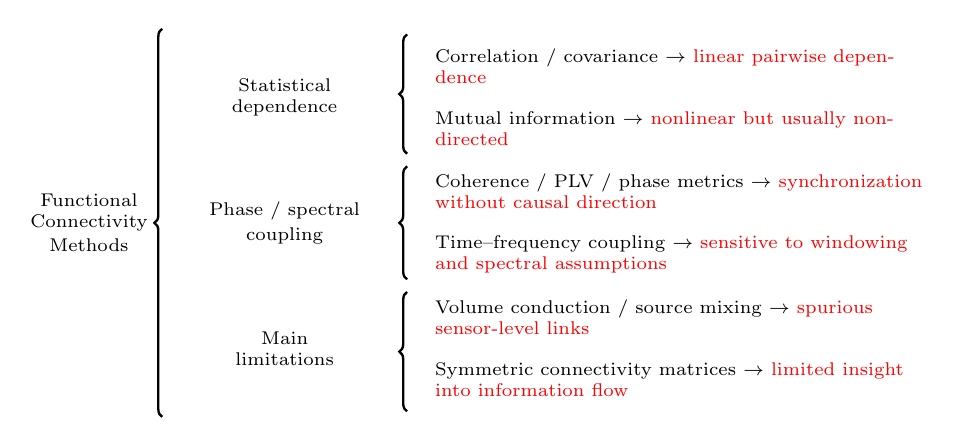
\begin{tikzpicture}[
  x=\linewidth, y=1.05cm, line width=0.85pt,
  font=\scriptsize,
  scale=0.95, every node/.style={transform shape}
]

% ===== spacing =====
\def\labelpad{0.012}
\def\topbotMain{0.07}
\def\topbotInner{0.00}
\def\dy{0.80}
\def\yT{2.00}
\def\amp{2.8pt}
\def\vgap{0.08}

% ===== styles =====
\tikzset{
  brace/.style={
    draw=none,
    postaction={draw,decorate,decoration={brace,mirror,raise=0pt,amplitude=\amp}}
  },
  lab/.style={anchor=east,fill=white,inner sep=1pt,align=center},
  glab/.style={anchor=center,fill=white,inner sep=1pt,align=center},
  item/.style={anchor=west,text width=0.55\linewidth,align=left}
}

% ===== column positions =====
\pgfmathsetmacro{\xMain}{0.25}
\pgfmathsetmacro{\xInner}{0.52}
\pgfmathsetmacro{\xText}{0.54}
\pgfmathsetmacro{\xMid}{(\xMain+\xInner)/2}

% ===== labels =====
\def\Main{\shortstack{Functional\\Connectivity\\Methods}}
\def\GOne{\shortstack{Statistical\\dependence}}
\def\GTwo{\shortstack{Phase / spectral\\coupling}}
\def\GThree{\shortstack{Main\\limitations}}

% ===== items =====
\def\Ione{Correlation / covariance $\rightarrow$ \textcolor{red}{linear pairwise dependence}}
\def\Itwo{Mutual information $\rightarrow$ \textcolor{red}{nonlinear but usually non-directed}}

\def\Ithree{Coherence / PLV / phase metrics $\rightarrow$ \textcolor{red}{synchronization without causal direction}}
\def\Ifour{Time--frequency coupling $\rightarrow$ \textcolor{red}{sensitive to windowing and spectral assumptions}}

\def\Ifive{Volume conduction / source mixing $\rightarrow$ \textcolor{red}{spurious sensor-level links}}
\def\Isix{Symmetric connectivity matrices $\rightarrow$ \textcolor{red}{limited insight into information flow}}

% ===== y positions =====
\pgfmathsetmacro{\yZero}{\yT}
\pgfmathsetmacro{\yOne}{\yT-1*\dy}
\pgfmathsetmacro{\yTwo}{\yT-2*\dy}
\pgfmathsetmacro{\yThree}{\yT-3*\dy}
\pgfmathsetmacro{\yFour}{\yT-4*\dy}
\pgfmathsetmacro{\yFive}{\yT-5*\dy}

% ===== main brace =====
\draw[brace] (\xMain,\yZero+0.5*\dy+\topbotMain) -- (\xMain,\yFive-0.5*\dy-\topbotMain);
\node[lab] at (\xMain-\labelpad,{(\yZero+\yFive)/2}) {\Main};

% ===== group braces =====
\draw[brace] (\xInner,\yZero+0.5*\dy+\topbotInner) --
             (\xInner,\yOne-0.5*\dy-\topbotInner+\vgap);

\draw[brace] (\xInner,\yTwo+0.5*\dy+\topbotInner-\vgap) --
             (\xInner,\yThree-0.5*\dy-\topbotInner+\vgap);

\draw[brace] (\xInner,\yFour+0.5*\dy+\topbotInner-\vgap) --
             (\xInner,\yFive-0.5*\dy-\topbotInner);

% ===== group labels =====
\node[glab] at (\xMid,{(\yZero+\yOne)/2}) {\GOne};
\node[glab] at (\xMid,{(\yTwo+\yThree)/2}) {\GTwo};
\node[glab] at (\xMid,{(\yFour+\yFive)/2}) {\GThree};

% ===== items =====
\node[item] at (\xText,\yZero) {\Ione};
\node[item] at (\xText,\yOne) {\Itwo};

\node[item] at (\xText,\yTwo) {\Ithree};
\node[item] at (\xText,\yThree) {\Ifour};

\node[item] at (\xText,\yFour) {\Ifive};
\node[item] at (\xText,\yFive) {\Isix};

\end{tikzpicture}

\vspace{0.4em}


\textbf{\scriptsize Relevant references:} 
{\scriptsize \cite{pereda2005nonlinear,bastos2016tutorial,vinck2011improved,faes2017information}}

\begin{center}
\centering\textcolor{frameblue}{
Functional connectivity captures statistical dependence between EEG signals, but it is often symmetric and sensitive to volume conduction and source mixing \cite{nagy2024spatial}
}
\end{center}

\end{frame}

% %--------------------------------------------

\begin{frame}{Effective Connectivity Methods for EEG-based BCI}
\centering

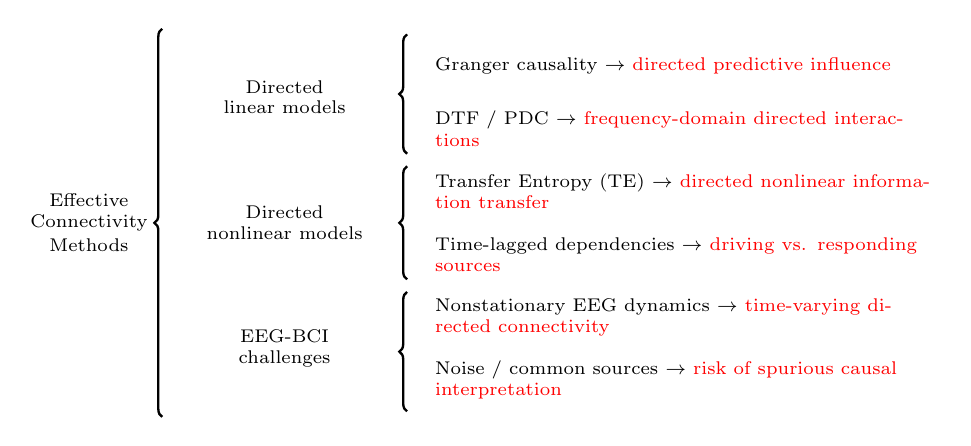
\begin{tikzpicture}[
  x=\linewidth, y=1.05cm, line width=0.85pt,
  font=\scriptsize,
  scale=0.95, every node/.style={transform shape}
]

% ===== spacing =====
\def\labelpad{0.012}
\def\topbotMain{0.07}
\def\topbotInner{0.00}
\def\dy{0.80}
\def\yT{2.00}
\def\amp{2.8pt}
\def\vgap{0.08}

% ===== styles =====
\tikzset{
  brace/.style={
    draw=none,
    postaction={draw,decorate,decoration={brace,mirror,raise=0pt,amplitude=\amp}}
  },
  lab/.style={anchor=east,fill=white,inner sep=1pt,align=center},
  glab/.style={anchor=center,fill=white,inner sep=1pt,align=center},
  item/.style={anchor=west,text width=0.55\linewidth,align=left}
}

% ===== column positions =====
\pgfmathsetmacro{\xMain}{0.25}
\pgfmathsetmacro{\xInner}{0.52}
\pgfmathsetmacro{\xText}{0.54}
\pgfmathsetmacro{\xMid}{(\xMain+\xInner)/2}

% ===== labels =====
\def\Main{\shortstack{Effective\\Connectivity\\Methods}}
\def\GOne{\shortstack{Directed\\linear models}}
\def\GTwo{\shortstack{Directed\\nonlinear models}}
\def\GThree{\shortstack{EEG-BCI\\challenges}}

% ===== items =====
\def\Ione{Granger causality $\rightarrow$ \textcolor{red}{directed predictive influence}}
\def\Itwo{DTF / PDC $\rightarrow$ \textcolor{red}{frequency-domain directed interactions}}

\def\Ithree{Transfer Entropy (TE) $\rightarrow$ \textcolor{red}{directed nonlinear information transfer}}
\def\Ifour{Time-lagged dependencies $\rightarrow$ \textcolor{red}{driving vs. responding sources}}

\def\Ifive{Nonstationary EEG dynamics $\rightarrow$ \textcolor{red}{time-varying directed connectivity}}
\def\Isix{Noise / common sources $\rightarrow$ \textcolor{red}{risk of spurious causal interpretation}}

% ===== y positions =====
\pgfmathsetmacro{\yZero}{\yT}
\pgfmathsetmacro{\yOne}{\yT-1*\dy}
\pgfmathsetmacro{\yTwo}{\yT-2*\dy}
\pgfmathsetmacro{\yThree}{\yT-3*\dy}
\pgfmathsetmacro{\yFour}{\yT-4*\dy}
\pgfmathsetmacro{\yFive}{\yT-5*\dy}

% ===== main brace =====
\draw[brace] (\xMain,\yZero+0.5*\dy+\topbotMain) -- (\xMain,\yFive-0.5*\dy-\topbotMain);
\node[lab] at (\xMain-\labelpad,{(\yZero+\yFive)/2}) {\Main};

% ===== group braces =====
\draw[brace] (\xInner,\yZero+0.5*\dy+\topbotInner) --
             (\xInner,\yOne-0.5*\dy-\topbotInner+\vgap);

\draw[brace] (\xInner,\yTwo+0.5*\dy+\topbotInner-\vgap) --
             (\xInner,\yThree-0.5*\dy-\topbotInner+\vgap);

\draw[brace] (\xInner,\yFour+0.5*\dy+\topbotInner-\vgap) --
             (\xInner,\yFive-0.5*\dy-\topbotInner);

% ===== group labels =====
\node[glab] at (\xMid,{(\yZero+\yOne)/2}) {\GOne};
\node[glab] at (\xMid,{(\yTwo+\yThree)/2}) {\GTwo};
\node[glab] at (\xMid,{(\yFour+\yFive)/2}) {\GThree};

% ===== items =====
\node[item] at (\xText,\yZero) {\Ione};
\node[item] at (\xText,\yOne) {\Itwo};

\node[item] at (\xText,\yTwo) {\Ithree};
\node[item] at (\xText,\yThree) {\Ifour};

\node[item] at (\xText,\yFour) {\Ifive};
\node[item] at (\xText,\yFive) {\Isix};

\end{tikzpicture}

\vspace{0.4em}

\textbf{ \scriptsize Relevant references:} 
{\scriptsize \cite{schreiber2000measuring,vicente2011transfer,faes2017information,zhou2025discovery}}

\begin{center}
\centering\textcolor{frameblue}{
Effective connectivity aims to estimate directed information flow in EEG, enabling nonlinear and time-lagged modeling of task-related interactions \cite{zhou2025discovery}
}
\end{center}

\end{frame}


%--------------------------------------------
% \subsection{Modeling Strategies for Inter- and Intra-subject Variability}

\begin{frame}{Modeling Strategies for Inter- and Intra-subject Variability}
\centering

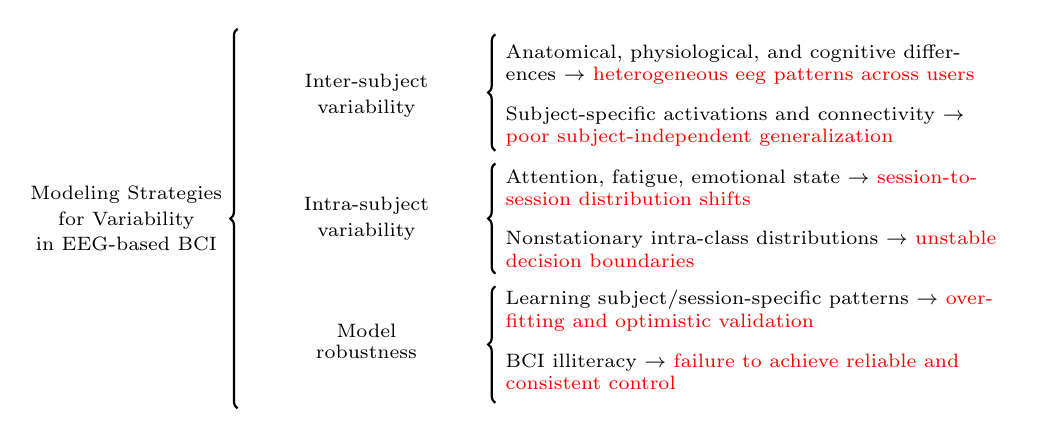
\begin{tikzpicture}[
  x=\linewidth, y=1.0cm, line width=0.8pt,
  font=\scriptsize,
  scale=1.0, every node/.style={transform shape}
]

% ===== spacing =====
\def\labelpad{0.012}
\def\topbotMain{0.07}
\def\topbotInner{0.00}
\def\dy{0.78}      % antes 1.1
\def\yT{2.05}      % baja el bloque
\def\amp{2.6pt}    % brace más pequeño
\def\vgap{0.08}    % menos separación entre braces

% ===== styles =====
\tikzset{
  brace/.style={
    draw=none,
    postaction={draw,decorate,decoration={brace,mirror,raise=0pt,amplitude=\amp}}
  },
  lab/.style={anchor=east,fill=white,inner sep=1pt,align=center},
  glab/.style={anchor=center,fill=white,inner sep=1pt,align=center},
  item/.style={anchor=west,text width=0.52\linewidth} % antes 0.58
}

% ===== column positions =====
\pgfmathsetmacro{\xMain}{0.26}
\pgfmathsetmacro{\xInner}{0.53}
\pgfmathsetmacro{\xText}{0.53}
\pgfmathsetmacro{\xMid}{(\xMain+\xInner)/2}

% ===== main label =====
\def\Main{\shortstack{Modeling Strategies\\for Variability\\in {EEG}-based {BCI}}}

% ===== group labels =====
\def\GOne{\shortstack{Inter-subject\\variability}}
\def\GTwo{\shortstack{Intra-subject\\variability}}
\def\GThree{\shortstack{Model\\robustness}}

% ===== items =====
\def\Ione{Anatomical, physiological, and cognitive differences $\rightarrow$ \textcolor{red}{heterogeneous {eeg} patterns across users}}
\def\Itwo{Subject-specific activations and connectivity $\rightarrow$ \textcolor{red}{poor subject-independent generalization}}

\def\Ithree{Attention, fatigue, emotional state $\rightarrow$ \textcolor{red}{session-to-session distribution shifts}}
\def\Ifour{Nonstationary intra-class distributions $\rightarrow$ \textcolor{red}{unstable decision boundaries}}

\def\Ifive{Learning subject/session-specific patterns $\rightarrow$ \textcolor{red}{overfitting and optimistic validation}}
\def\Isix{{BCI} illiteracy $\rightarrow$ \textcolor{red}{failure to achieve reliable and consistent control}}

% ===== y positions =====
\pgfmathsetmacro{\yZero}{\yT}
\pgfmathsetmacro{\yOne}{\yT-1*\dy}
\pgfmathsetmacro{\yTwo}{\yT-2*\dy}
\pgfmathsetmacro{\yThree}{\yT-3*\dy}
\pgfmathsetmacro{\yFour}{\yT-4*\dy}
\pgfmathsetmacro{\yFive}{\yT-5*\dy}

% ===== main brace =====
\draw[brace] (\xMain,\yZero+0.5*\dy+\topbotMain) -- (\xMain,\yFive-0.5*\dy-\topbotMain);
\node[lab] at (\xMain-\labelpad,{(\yZero+\yFive)/2}) {\Main};

% ===== group braces =====
\draw[brace] (\xInner,\yZero+0.5*\dy+\topbotInner) --
             (\xInner,\yOne-0.5*\dy-\topbotInner+\vgap);

\draw[brace] (\xInner,\yTwo+0.5*\dy+\topbotInner-\vgap) --
             (\xInner,\yThree-0.5*\dy-\topbotInner+\vgap);

\draw[brace] (\xInner,\yFour+0.5*\dy+\topbotInner-\vgap) --
             (\xInner,\yFive-0.5*\dy-\topbotInner);

% ===== group labels =====
\node[glab] at (\xMid,{(\yZero+\yOne)/2}) {\GOne};
\node[glab] at (\xMid,{(\yTwo+\yThree)/2}) {\GTwo};
\node[glab] at (\xMid,{(\yFour+\yFive)/2}) {\GThree};

% ===== items =====
\node[item] at (\xText,\yZero) {\Ione};
\node[item] at (\xText,\yOne) {\Itwo};

\node[item] at (\xText,\yTwo) {\Ithree};
\node[item] at (\xText,\yThree) {\Ifour};

\node[item] at (\xText,\yFour) {\Ifive};
\node[item] at (\xText,\yFive) {\Isix};

\end{tikzpicture}

\vspace{0.4em}

\textbf{\scriptsize Relevant references:} 
\cite{kim2023bridging,maswanganyi2022statistical,saha2020intra,duang,Raza}
\begin{center}
    \centering\textcolor{frameblue}{EEG-BCI performance is limited by inter-/intra-subject variability, causing distribution shifts, overfitting, and poor subject-independent generalization \cite{sartipi2024subject}}
\end{center}

\end{frame}

%--------------------------------------------
% \subsection{Interpretability in EEG-based Deep Learning}
\begin{frame}{Interpretability in EEG-based Deep Learning}
\centering

% --- Versión más compacta (8 ítems: toca apretar más) ---
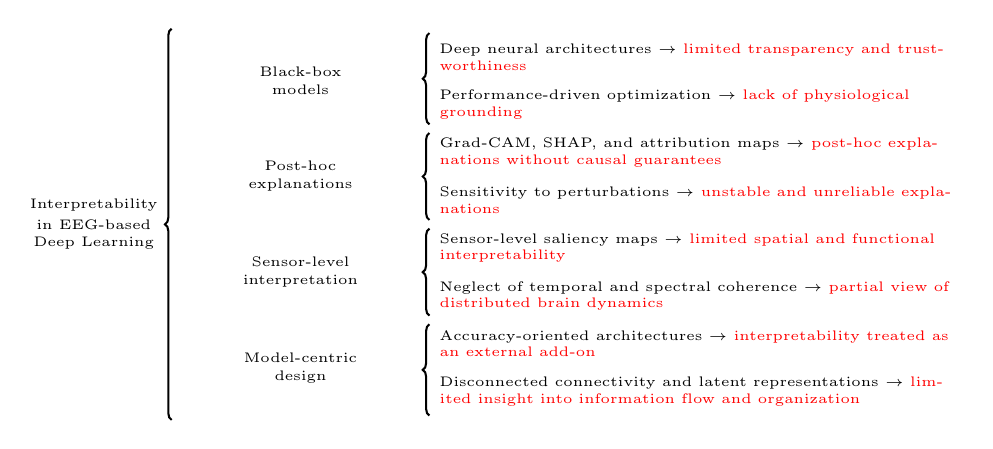
\begin{tikzpicture}[
  x=\linewidth, y=0.92cm, line width=0.75pt,
  font=\tiny,
  scale=1.0, every node/.style={transform shape}
]

% ===== spacing =====
\def\labelpad{0.011}
\def\topbotMain{0.06}
\def\topbotInner{0.00}
\def\dy{0.66}       % antes 1.0 (MUCHO más compacto)
\def\yT{2.05}       % ajusta inicio
\def\amp{2.4pt}
\def\vgap{0.06}

% ===== styles =====
\tikzset{
  brace/.style={
    draw=none,
    postaction={draw,decorate,decoration={brace,mirror,raise=0pt,amplitude=\amp}}
  },
  lab/.style={anchor=east,fill=white,inner sep=0.9pt,align=center},
  glab/.style={anchor=center,fill=white,inner sep=0.9pt,align=center},
  item/.style={anchor=west,text width=0.54\linewidth} % un poco menor
}

% ===== column positions =====
\pgfmathsetmacro{\xMain}{0.25}
\pgfmathsetmacro{\xInner}{0.52}
\pgfmathsetmacro{\xText}{0.52}
\pgfmathsetmacro{\xMid}{(\xMain+\xInner)/2}

% ===== main label =====
\def\Main{\shortstack{Interpretability\\in EEG-based\\Deep Learning}}

% ===== group labels =====
\def\GOne{\shortstack{Black-box\\models}}
\def\GTwo{\shortstack{Post-hoc\\explanations}}
\def\GThree{\shortstack{Sensor-level\\interpretation}}
\def\GFour{\shortstack{Model-centric\\design}}

% ===== items (compactos en una sola línea) =====
\def\Ione{Deep neural architectures $\rightarrow$ \textcolor{red}{limited transparency and trustworthiness}}
\def\Itwo{Performance-driven optimization $\rightarrow$ \textcolor{red}{lack of physiological grounding}}

\def\Ithree{Grad-CAM, SHAP, and attribution maps $\rightarrow$ \textcolor{red}{post-hoc explanations without causal guarantees}}
\def\Ifour{Sensitivity to perturbations $\rightarrow$ \textcolor{red}{unstable and unreliable explanations}}

\def\Ifive{Sensor-level saliency maps $\rightarrow$ \textcolor{red}{limited spatial and functional interpretability}}
\def\Isix{Neglect of temporal and spectral coherence $\rightarrow$ \textcolor{red}{partial view of distributed brain dynamics}}

\def\Iseven{Accuracy-oriented architectures $\rightarrow$ \textcolor{red}{interpretability treated as an external add-on}}
\def\Ieight{Disconnected connectivity and latent representations $\rightarrow$ \textcolor{red}{limited insight into information flow and organization}}

% ===== y positions =====
\pgfmathsetmacro{\yZero}{\yT}
\pgfmathsetmacro{\yOne}{\yT-1*\dy}
\pgfmathsetmacro{\yTwo}{\yT-2*\dy}
\pgfmathsetmacro{\yThree}{\yT-3*\dy}
\pgfmathsetmacro{\yFour}{\yT-4*\dy}
\pgfmathsetmacro{\yFive}{\yT-5*\dy}
\pgfmathsetmacro{\ySix}{\yT-6*\dy}
\pgfmathsetmacro{\ySeven}{\yT-7*\dy}

% ===== main brace =====
\draw[brace] (\xMain,\yZero+0.5*\dy+\topbotMain) -- (\xMain,\ySeven-0.5*\dy-\topbotMain);
\node[lab] at (\xMain-\labelpad,{(\yZero+\ySeven)/2}) {\Main};

% ===== group braces =====
\draw[brace] (\xInner,\yZero+0.5*\dy+\topbotInner) --
             (\xInner,\yOne-0.5*\dy-\topbotInner+\vgap);

\draw[brace] (\xInner,\yTwo+0.5*\dy+\topbotInner-\vgap) --
             (\xInner,\yThree-0.5*\dy-\topbotInner+\vgap);

\draw[brace] (\xInner,\yFour+0.5*\dy+\topbotInner-\vgap) --
             (\xInner,\yFive-0.5*\dy-\topbotInner+\vgap);

\draw[brace] (\xInner,\ySix+0.5*\dy+\topbotInner-\vgap) --
             (\xInner,\ySeven-0.5*\dy-\topbotInner);

% ===== group labels =====
\node[glab] at (\xMid,{(\yZero+\yOne)/2}) {\GOne};
\node[glab] at (\xMid,{(\yTwo+\yThree)/2}) {\GTwo};
\node[glab] at (\xMid,{(\yFour+\yFive)/2}) {\GThree};
\node[glab] at (\xMid,{(\ySix+\ySeven)/2}) {\GFour};

% ===== items =====
\node[item] at (\xText,\yZero) {\Ione};
\node[item] at (\xText,\yOne) {\Itwo};

\node[item] at (\xText,\yTwo) {\Ithree};
\node[item] at (\xText,\yThree) {\Ifour};

\node[item] at (\xText,\yFour) {\Ifive};
\node[item] at (\xText,\yFive) {\Isix};

\node[item] at (\xText,\ySix) {\Iseven};
\node[item] at (\xText,\ySeven) {\Ieight};
\end{tikzpicture}

\vspace{0.4em}

\textbf{ \scriptsize Relevant references:} 
\cite{sturm2016interpretable,Selvaraju2016,liu2023cam,ahmed2023,liu2023multiattention,collazos2023posthoc}

\begin{center}
    \centering\textcolor{frameblue}{Interpretability in EEG deep learning remains limited, relying on black-box models and unstable post-hoc explanations with weak neurophysiological grounding \cite{zhou2024interpretable_robust_eeg}}
\end{center}
\end{frame}

%--------------------------------------------
\section{Aims}

\begin{frame}{General Aim}

   \begin{itemize}
\justifying
   \item To develop an \textbf{interpretable} deep learning framework for {EEG-based BCI systems} that addresses the challenges of \textbf{low spatial resolution} and \textbf{noise sensitivity}, \textbf{nonlinear} and \textbf{nonstationary} brain dynamics, and \textbf{high inter} and \textbf{intra-subject variability}, with the goal of improving generalization  \textbf{across subjects and sessions}, and \textbf{neurophysiological interpretability} in {real-world classification scenarios}.

   \end{itemize}
\end{frame}

%--------------------------------------------
\begin{frame}{Specific Aims}
  \begin{itemize}
    \setlength\itemsep{0.4em}
    \justifying

    \item[1] To design a representation learning strategy that mitigates the effects of 
    \textbf{low spatial resolution} and \textbf{noise} induced by \textbf{volume conduction} 
    and \textbf{physiological artifacts}, by incorporating {spatio-temporal} 
    representations from {multi-channel} data to support 
    {EEG-based classification tasks}.
    
    \item[2] To design a \textbf{dynamical connectivity learning} strategy that captures 
    \textbf{nonlinear}, \textbf{non-stationary}, \textbf{time-delayed}, and 
    \textbf{directed} EEG channel dependencies, by incorporating 
    {state-space temporal representations} and {information-theoretic connectivity measures} from {multi-channel} data 
    to characterize {task-related directed brain interactions}.

    \item[3] To develop an \textbf{interpretable} Deep Learning Based EEG classification approach 
    that includes directed-connectivity measures to code \textbf{nonlinear} and 
    \textbf{nonstationary} {EEG channel dependencies}, enabling the characterization 
    of {time-varying brain interactions} across {cognitive and neurophysiological} processes for \textbf{subject-dependent} and \textbf{subject-independent} scenarios.

  \end{itemize}
\end{frame}

%--------------------------------------------
% \section{Contributions}
% \begin{frame}{Outline and Contributions}

% \begin{figure}
%     \centering
%     \includegraphics[width=0.5\linewidth]{figures/contributions.pdf}
% \end{figure}

% \centering
% {\color{frameblue}
%  This doctoral research integrates functional connectivity, effective connectivity, and attention-based learning to improve robustness, generalization, and interpretability \\ in EEG decoding
% }

% \end{frame}
%--------------------------------------------
\section{Datasets}
%--------------------------------------------
\begin{frame}{EEG Datasets}

% \scriptsize

\begin{columns}[T,totalwidth=\textwidth]

%==================================================
% GIGASCIENCE
%==================================================
\begin{column}{0.48\textwidth}
\centering
\textbf{\normalsize GigaScience MI-EEG} {\scriptsize (Cho et al., 2017)}

\vspace{0.10cm}

\makebox[\linewidth][c]{%
\begin{minipage}{0.35\linewidth}
    \centering
    \resizebox{2.5cm}{!}{% Color definitions (RGB format)
\definecolor{UpperGreen}{RGB}{145,209,200}     % #91d1c8
\definecolor{LowerGreen}{RGB}{179,223,106}     % #b3df6a
\definecolor{Red}{RGB}{251,129,113}            % #fb8171
\definecolor{YellowR}{RGB}{255,254,178}        % #fffeb2
\definecolor{GrayL}{RGB}{217,216,217}          % #d9d8d9
\definecolor{Orange}{RGB}{252,181,98}          % #fcb562
\definecolor{GreenL}{RGB}{205,235,197}         % #cdebc5
\definecolor{YellowL}{RGB}{255,236,108}        % #ffec6c
\definecolor{ElecBG}{RGB}{207,231,226}         % #CFE7E2

% Parameters - Centralized for easy modification
\def\radiusX{1.2}
\def\radiusY{1.2}

\def\earWidth{0.08}
\def\earHeight{0.30}
\def\earOffset{1.225}

\def\noseBase{0.485}
\def\noseHeight{0.380}
\def\noseTip{0.05}
\def\sep{0.215}

% Electrode style
\tikzset{
  electrode/.style={
    draw,
    line width=0.5pt,
    circle,
    inner sep=1pt,
    minimum size=6mm,
    fill=ElecBG!50!white,
    fill opacity=0.85,
    font=\scriptsize,
    text opacity=1
  }
}

\begin{tikzpicture}[scale=3.25]
    %%% Nose
    \draw[line width=1pt]
      ($(0,1)+(-\noseBase,-\noseTip)$) -- 
      ($(0,1)+(0,\noseHeight)$) -- 
      ($(0,1)+(\noseBase,-\noseTip)$) -- cycle;

    %%% Ears
    \draw[line width=1pt] ($(0,0.0)+(180:\earOffset)$) ellipse ({\earWidth} and {\earHeight});
    \draw[line width=1pt] ($(0,0.0)+(0:\earOffset)$) ellipse ({\earWidth} and {\earHeight});

    %%% Head outline
    \filldraw[fill=white,draw=black,line width=1pt] (0,0) ellipse ({\radiusX} and {\radiusY});
    
    %%% Define electrode positions FIRST (invisible, just coordinates)
    \coordinate (Cz) at (90:0.0); 
    
    % Vertical midline electrodes
    \coordinate (FPz) at ($(Cz)+(0,1.125*5.0*\sep)$);
    \coordinate (AFz) at ($(Cz)+(0,1.125*3.75*\sep)$);
    \coordinate (Fz) at ($(Cz)+(0,1.125*2.50*\sep)$);
    \coordinate (FCz) at ($(Cz)+(0,1.125*1.25*\sep)$);

    \coordinate (CPz) at ($(Cz)+(0,1.125*-1.25*\sep)$);
    \coordinate (Pz) at ($(Cz)+(0,1.125*-2.50*\sep)$);
    \coordinate (POz) at ($(Cz)+(0,1.125*-3.75*\sep)$);
    \coordinate (Oz) at ($(Cz)+(0,1.125*-5.0*\sep)$);
    \coordinate (Iz) at ($(Cz)+(0,1.125*-6.25*\sep)$);
    
    % Vertical left midline
    \coordinate (F1) at ($(Oz)+(-1.125*\sep,182*0.01)$);
    \coordinate (F3) at ($(Oz)+(-2.25*\sep,184*0.01)$);
    \coordinate (F5) at ($(Oz)+(-3.375*\sep,187*0.01)$);
    \coordinate (F7) at ($(Oz)+(-4.5*\sep,200*0.01)$);
    
    \coordinate (AF3) at ($(Oz)+(-1.8*\sep,215*0.01)$);
    \coordinate (AF7) at ($(Oz)+(-3.15*\sep,225*0.01)$);
    
    \coordinate (FP1) at ($(Oz)+(-1.75*\sep,240*0.01)$);

    % Vertical right midline
    \coordinate (F2) at ($(Oz)+(1.125*\sep,182*0.01)$);
    \coordinate (F4) at ($(Oz)+(2.25*\sep,184*0.01)$);
    \coordinate (F6) at ($(Oz)+(3.375*\sep,187*0.01)$);
    \coordinate (F8) at ($(Oz)+(4.5*\sep,200*0.01)$);
    
    \coordinate (AF4) at ($(Oz)+(1.8*\sep,215*0.01)$);
    \coordinate (AF8) at ($(Oz)+(3.25*\sep,225*0.01)$);
    
    \coordinate (FP2) at ($(Oz)+(1.75*\sep,240*0.01)$);
    
    % Horizontal right electrodes
    \coordinate (C2) at ($(Cz)+(1.375*\sep,0)$);
    \coordinate (C4) at ($(Cz)+(2.75*\sep,0)$);
    \coordinate (C6) at ($(Cz)+(4.125*\sep,0)$);
    \coordinate (T8) at ($(Cz)+(5.5*\sep,0)$);
    
    % Horizontal left electrodes
    \coordinate (C1) at ($(Cz)+(-1.375*\sep,0)$);
    \coordinate (C3) at ($(Cz)+(-2.75*\sep,0)$);
    \coordinate (C5) at ($(Cz)+(-4.125*\sep,0)$);
    \coordinate (T7) at ($(Cz)+(-5.5*\sep,0)$);
    
    % Lower right electrodes
    \coordinate (CP2) at ($(Oz)+(1.35*\sep,91*0.01)$);
    \coordinate (CP4) at ($(Oz)+(2.7*\sep,88*0.01)$);
    \coordinate (CP6) at ($(Oz)+(4.05*\sep,85*0.01)$);
    \coordinate (TP8) at ($(Oz)+(5.40*\sep,78*0.01)$);
    
    \coordinate (P2) at ($(Oz)+(1.05*\sep,61*0.01)$);
    \coordinate (P4) at ($(Oz)+(2.1*\sep,59*0.01)$);
    \coordinate (P6) at ($(Oz)+(3.15*\sep,55*0.01)$);
    \coordinate (P8) at ($(Oz)+(4.2*\sep,47*0.01)$);
    \coordinate (P10) at ($(Oz)+(5.25*\sep,37*0.01)$);
    
    \coordinate (PO4) at ($(Oz)+(1.8*\sep,29*0.01)$);
    \coordinate (PO8) at ($(Oz)+(3.25*\sep,17.5*0.01)$);

    \coordinate (O2) at ($(Oz)+(1.75*\sep,2*0.01)$);
    
    % Lower left electrodes
    \coordinate (CP1) at ($(Oz)+(-1.35*\sep,91*0.01)$);
    \coordinate (CP3) at ($(Oz)+(-2.7*\sep,88*0.01)$);
    \coordinate (CP5) at ($(Oz)+(-4.05*\sep,85*0.01)$);
    \coordinate (TP7) at ($(Oz)+(-5.40*\sep,78*0.01)$);
    
    \coordinate (P1) at ($(Oz)+(-1.05*\sep,61*0.01)$);
    \coordinate (P3) at ($(Oz)+(-2.1*\sep,59*0.01)$);
    \coordinate (P5) at ($(Oz)+(-3.15*\sep,55*0.01)$);
    \coordinate (P7) at ($(Oz)+(-4.2*\sep,47*0.01)$);
    \coordinate (P9) at ($(Oz)+(-5.25*\sep,37*0.01)$);

    \coordinate (PO3) at ($(Oz)+(-1.8*\sep,29*0.01)$);
    \coordinate (PO7) at ($(Oz)+(-3.25*\sep,17.5*0.01)$);

    \coordinate (O1) at ($(Oz)+(-1.75*\sep,2*0.01)$);
    
    % Upper right electrodes
    \coordinate (FC2) at ($(Oz)+(1.35*\sep,152*0.01)$);
    \coordinate (FC4) at ($(Oz)+(2.70*\sep,154.5*0.01)$);
    \coordinate (FC6) at ($(Oz)+(4.05*\sep,158.5*0.01)$);
    \coordinate (FT8) at ($(Oz)+(5.40*\sep,164.5*0.01)$);
    
    % Upper left electrodes
    \coordinate (FC1) at ($(Oz)+(-1.35*\sep,152*0.01)$);
    \coordinate (FC3) at ($(Oz)+(-2.70*\sep,154*0.01)$);
    \coordinate (FC5) at ($(Oz)+(-4.05*\sep,158*0.01)$);
    \coordinate (FT7) at ($(Oz)+(-5.40*\sep,164.5*0.01)$);

    %%% Right regions (Yellow - Orange - Red)
    \begin{pgfonlayer}{main}
        \begin{scope}
            \clip (0,0) ellipse ({\radiusX} and {-\radiusY});
            \fill[Red] ($(Fz)+(0,0)$) rectangle (\radiusX,-\radiusY);
        \end{scope}
    \end{pgfonlayer}

    \begin{pgfonlayer}{main}
        \begin{scope}
            \clip (0,0) ellipse ({\radiusX} and {-\radiusY});
            \fill[YellowR] ($(Fz)+(0,-0.125)$) rectangle (\radiusX,\radiusY);
        \end{scope}
    \end{pgfonlayer}

    \begin{pgfonlayer}{main}
        \begin{scope}
            \clip (0,0) ellipse ({\radiusX} and {-\radiusY});
            \fill[Orange] ($(Pz)+(0,0.125)$) rectangle (\radiusX,-\radiusY);
        \end{scope}
    \end{pgfonlayer}

    %%% Left regions (Green - Yellow - Gray)
    \begin{pgfonlayer}{main}
        \begin{scope}
            \clip (0,0) ellipse ({\radiusX} and {-\radiusY});
            \fill[GreenL] ($(Fz)+(0,0)$) rectangle (-\radiusX,-\radiusY);
        \end{scope}
    \end{pgfonlayer}

    \begin{pgfonlayer}{main}
        \begin{scope}
            \clip (0,0) ellipse ({\radiusX} and {-\radiusY});
            \fill[YellowL] ($(Fz)+(0,-0.125)$) rectangle (-\radiusX,\radiusY);
        \end{scope}
    \end{pgfonlayer}

    \begin{pgfonlayer}{main}
        \begin{scope}
            \clip (0,0) ellipse ({\radiusX} and {-\radiusY});
            \fill[GrayL] ($(Pz)+(0,0.125)$) rectangle (-\radiusX,-\radiusY);
        \end{scope}
    \end{pgfonlayer}

    %%% Upper Green region
    \coordinate (Lmid) at ($(Cz)!0.415!(C1)$);
    \coordinate (Rmid) at ($(Cz)!0.415!(C2)$);
    \coordinate (TopMid) at ($(Cz)!0.415!(FCz)$);
    
    \path[name path=rim] (0,0) ellipse ({\radiusX} and {\radiusY});
    \path[name path=vertL] ($(Lmid)+(0,5)$) -- ($(Lmid)+(0,-5)$);
    \path[name path=vertR] ($(Rmid)+(0,5)$) -- ($(Rmid)+(0,-5)$);
    
    \path[name intersections={of=vertL and rim, by={TL,BL}}];
    \path[name intersections={of=vertR and rim, by={TR,BR}}];
    
    \begin{pgfonlayer}{main}
      \begin{scope}
        \clip (0,0) ellipse ({\radiusX} and {\radiusY});
        \fill[UpperGreen]
          (TL) to[out=90,in=90,looseness=1.3] (TR) --
          ($(TR)+(0,-1.5)$) --
          ($(TL)+(0,-1.5)$) -- cycle;
      \end{scope}
    \end{pgfonlayer}
           
    %%% Lower Green region
    \path[name intersections={of=vertL and rim, by={UL,DL}}];
    \path[name intersections={of=vertR and rim, by={UR,DR}}];
    
    \coordinate (MidDown) at ($(FCz)!0.415!(Cz)$);
    \coordinate (BL2) at ($(Lmid |- MidDown)$);
    \coordinate (BR2) at ($(Rmid |- MidDown)$);
    
    \begin{pgfonlayer}{foreground}
        \fill[LowerGreen] (BL2) -- (BR2) -- (DR) -- (DL) -- cycle;
    \end{pgfonlayer}
    
    \begin{pgfonlayer}{main}
        \begin{scope}
            \clip (0,0) ellipse ({\radiusX} and {\radiusY});
            \fill[LowerGreen]
                ($(POz)+(-0.1,0)$) --
                ($(POz)+(0.1,0)$) --
                ($(0,-2)+(0.7,0)$) --
                ($(0,-2)+(-0.7,0)$) -- cycle;
        \end{scope}
        
    \end{pgfonlayer}

    \begin{pgfonlayer}{foreground}
            % Central electrode
    \node[electrode] at (Cz) {Cz}; 
    
    % Vertical midline electrodes
    \node[electrode] at (FPz) {FPz};
    \node[electrode] at (AFz) {AFz};
    \node[electrode] at (Fz) {Fz};
    \node[electrode] at (FCz) {FCz};
 
    % Vertical left midline
    \node[electrode] at (F1) {F1};
    \node[electrode] at (F3) {F3};
    \node[electrode] at (F5) {F5};
    \node[electrode] at (F7) {F7};
    \node[electrode] at (AF3) {AF3};
    \node[electrode] at (AF7) {AF7};
    \node[electrode] at (FP1) {FP1};
      
    % Vertical right midline
    \node[electrode] at (F2) {F2};
    \node[electrode] at (F4) {F4};
    \node[electrode] at (F6) {F6};
    \node[electrode] at (F8) {F8};
    \node[electrode] at (AF4) {AF4};
    \node[electrode] at (AF8) {AF8};
    \node[electrode] at (FP2) {FP2};
    
      % Horizontal right electrodes
      \node[electrode] at (C2) {C2};
      \node[electrode] at (C4) {C4};
      \node[electrode] at (C6) {C6};
      \node[electrode] at (T8) {T8};
      
    % Horizontal left electrodes
    \node[electrode] at (C1) {C1};
    \node[electrode] at (C3) {C3};
    \node[electrode] at (C5) {C5};
    \node[electrode] at (T7) {T7};
    
    % Lower right electrodes
    \node[electrode] at (CP2) {CP2};
    \node[electrode] at (CP4) {CP4};
    \node[electrode] at (CP6) {CP6};
    \node[electrode] at (TP8) {TP8};

    \node[electrode] at (P2) {P2};
    \node[electrode] at (P4) {P4};
    \node[electrode] at (P6) {P6};
    \node[electrode] at (P8) {P8};
    \node[electrode] at (P10) {P10};

    \node[electrode] at (PO4) {PO4};
    \node[electrode] at (PO8) {PO8};

    \node[electrode] at (O2) {O2};

    % Lower left electrodes
    \node[electrode] at (CP1) {CP1};
    \node[electrode] at (CP3) {CP3};
    \node[electrode] at (CP5) {CP5};
    \node[electrode] at (TP7) {TP7};
      
    \node[electrode] at (P1) {P1};
    \node[electrode] at (P3) {P3};
    \node[electrode] at (P5) {P5};
    \node[electrode] at (P7) {P7};
    \node[electrode] at (P9) {P9};
      
    \node[electrode] at (PO3) {PO3};
    \node[electrode] at (PO7) {PO7};

    \node[electrode] at (O1) {O1};
    
    % Upper right electrodes
    \node[electrode] at (FC2) {FC2};
    \node[electrode] at (FC4) {FC4};
    \node[electrode] at (FC6) {FC6};
    \node[electrode] at (FT8) {FT8};
    
    % Upper left electrodes
    \node[electrode] at (FC1) {FC1};
    \node[electrode] at (FC3) {FC3};
    \node[electrode] at (FC5) {FC5};
    \node[electrode] at (FT7) {FT7};
      
    \node[electrode] at (CPz) {CPz};
    \node[electrode] at (Pz) {Pz};
    \node[electrode] at (POz) {POz};
    \node[electrode] at (Oz) {Oz};
    \node[electrode] at (Iz) {Iz};
      
    %%% Reset bounding box
    \pgfresetboundingbox
    \path (0,-1.305*\radiusY) (0,1.115*\radiusY) (-1.05*\radiusX,0) (1.05*\radiusX,0);
    \end{pgfonlayer}
    
\end{tikzpicture}}
    
\end{minipage}
\hspace{0.15cm}
\begin{minipage}{0.55\linewidth}
    \centering
    \resizebox{4.4cm}{!}{% Paleta pastel alternativa (nuevos matices)
\definecolor{FixationColor}{HTML}{BFD8B8} % sage
\definecolor{MotorColor}{HTML}{F6C28B}    % peach/sand
\definecolor{RestColor}{HTML}{A7C5EB}     % powder blue
\definecolor{InterColor}{HTML}{EDE6F2}    % mist lavender-gray
\definecolor{CueColor}{HTML}{B5EAEA}      % mint

\begin{tikzpicture}
  % ===== Parámetros =====
  \def\boxheight{2.2}
  \def\startFix{-2}
  \def\endFix{0}
  \def\endCue{1}      % Duración del cue (0–1 s). Cambia a 0.8 si lo quieres más corto
  \def\endMI{3}
  \def\endRest{5}
  \def\endInter{5.8}

  \def\plusLen{0.18}  % Tamaño de la cruz (+); baja este valor para hacerla más pequeña
  \def\showPlusInRest{1} % 1=mostrar cruz en Rest, 0=ocultar

  % ===== Bloques =====
  \fill[FixationColor] (\startFix,0) rectangle (\endFix,\boxheight);
  % MI SIN cruce con cue: inicia en 1 s
  \fill[MotorColor]    (\endCue,0)   rectangle (\endMI,\boxheight);
  \fill[RestColor]     (\endMI,0)    rectangle (\endRest,\boxheight);
  \fill[InterColor]    (\endRest,0)  rectangle (\endInter,\boxheight);
  % Cue como bloque vertical (0–1 s)
  \fill[CueColor]      (\endFix,0)   rectangle (\endCue,\boxheight);

  % ===== Etiquetas =====
  \node[font=\small]              at ({(\startFix+\endFix)/2},{0.5*\boxheight}) {Fixation};
  \node[font=\small,align=center] at ({(\endCue+\endMI)/2},{0.5*\boxheight}) {EEG Motor\\Movement/\\MI};
  \node[font=\small]              at ({(\endMI+\endRest)/2},{0.5*\boxheight}) {Rest};
  \node[font=\footnotesize,rotate=90]
       at ({(\endRest+\endInter)/2},{0.5*\boxheight}) {\shortstack{Inter-trials\\0.1--0.8\,s}};
  \node[font=\small]              at ({(\endFix+\endCue)/2},{0.5*\boxheight}) {Cue};

  % ===== Cruces (+) =====
  % Fixation
  \pgfmathsetmacro{\xfix}{(\startFix+\endFix)/2}
  \pgfmathsetmacro{\yfix}{0.68*\boxheight}
  \draw[line width=0.8pt] (\xfix,\yfix-\plusLen) -- (\xfix,\yfix+\plusLen);
  \draw[line width=0.8pt] (\xfix-\plusLen,\yfix) -- (\xfix+\plusLen,\yfix);

  % Rest (opcional)
  \ifnum\showPlusInRest=1
    \pgfmathsetmacro{\xrest}{(\endMI+\endRest)/2}
    \pgfmathsetmacro{\yrest}{0.68*\boxheight}
    \draw[line width=0.8pt] (\xrest,\yrest-\plusLen) -- (\xrest,\yrest+\plusLen);
    \draw[line width=0.8pt] (\xrest-\plusLen,\yrest) -- (\xrest+\plusLen,\yrest);
  \fi

  % ===== Eje X =====
  \draw[thick] (\startFix,0) -- (\endInter,0) node[below right,font=\small] {Time [s]};
  \foreach \x/\lbl in {\startFix/-2, 0/0, \endMI/3, \endRest/5}{
    \draw (\x,0) -- ++(0,-2pt) node[below,font=\footnotesize] {\lbl};
  }

\end{tikzpicture}}
    
\end{minipage}
}

\vspace{0.12cm}

\raggedright
\begin{itemize}\itemsep1pt
    \item 50 subjects, 64 channels, 128 Hz
    \item Left- vs. right-hand MI
    \item Butterworth band-pass: 4--40 Hz
    \item Window: 0.5--2.5 s post-cue
\end{itemize}

\end{column}

%==================================================
% BCI IV-2A
%==================================================
\begin{column}{0.48\textwidth}
\centering
\textbf{\normalsize BCI Competition IV-2a} {\scriptsize (Tangermann et al., 2012)}


\makebox[\linewidth][c]{%
\begin{minipage}{0.35\linewidth}
    \centering
    \resizebox{3.0cm}{!}{\definecolor{UpperGreen}{HTML}{8DD3C8}
\definecolor{LowerYellow}{HTML}{FEFFB3}
\definecolor{BlueRightSide}{HTML}{80B0D3}
\definecolor{PurpleLeftSide}{HTML}{BD80BD}
\definecolor{Purple}{HTML}{BFBADA} 
\definecolor{GrayC}{HTML}{D8D8D9} 
\definecolor{Orange}{HTML}{FDB463}
\definecolor{GreenC}{HTML}{CDEBC4}
\definecolor{GreenD}{HTML}{B2DF6A}
\definecolor{YellowC}{HTML}{FEEC6F}
\definecolor{ElecBG}{HTML}{CFE7E2}

%%% Parameters - Centralized for easy modification
\def\radiusX{1.0}
\def\radiusY{1.0}
\def\earWidth{0.08}
\def\earHeight{0.35}
\def\earOffset{1.1}
\def\noseBase{0.30}
\def\noseHeight{0.15}
\def\noseTip{0.05}
\def\sep{0.275}

%%% Electrode style
\tikzset{
  electrode/.style={
    draw,
    line width=0.5pt,
    circle,
    inner sep=1pt,
    minimum size=6mm,
    fill=ElecBG!50!white,
    fill opacity=0.85,
    font=\scriptsize,
    text opacity=1
  }
}



\begin{tikzpicture}[scale=3]

    %%% Nose
    \draw[line width=1pt]
      ($(0,1)+(-\noseBase,-\noseTip)$) -- 
      ($(0,1)+(0,\noseHeight)$) -- 
      ($(0,1)+(\noseBase,-\noseTip)$) -- cycle;

    %%% Ears
    \draw[line width=1pt] ($(0.085,0.05)+(180:\earOffset)$) ellipse ({\earWidth} and {\earHeight});
    \draw[line width=1pt] ($(-0.085,0.05)+(0:\earOffset)$) ellipse ({\earWidth} and {\earHeight});
    
    %%% Head outline
    \filldraw[fill=white,draw=black,line width=1pt] (0,0) ellipse ({\radiusX} and {\radiusY});
    
    %%% Define electrode positions FIRST (invisible, just coordinates)
    \coordinate (Cz) at (90:0.1); 
    
    % Vertical midline electrodes
    \coordinate (FCz) at ($(Cz)+(0,1*\sep)$);
    \coordinate (Fz) at ($(Cz)+(0,2*\sep)$);
    \coordinate (CPz) at ($(Cz)+(0,-1*\sep)$);
    \coordinate (Pz) at ($(Cz)+(0,-2*\sep)$);
    \coordinate (POz) at ($(Cz)+(0,-3*\sep)$);
    
    % Horizontal right electrodes
    \coordinate (C2) at ($(Cz)+(1*\sep,0)$);
    \coordinate (C4) at ($(Cz)+(2*\sep,0)$);
    \coordinate (C6) at ($(Cz)+(3*\sep,0)$);
    
    % Horizontal left electrodes
    \coordinate (C1) at ($(Cz)+(-1*\sep,0)$);
    \coordinate (C3) at ($(Cz)+(-2*\sep,0)$);
    \coordinate (C5) at ($(Cz)+(-3*\sep,0)$);
    
    % Lower right electrodes
    \coordinate (CP2) at ($(CPz)+(1*\sep,0)$);
    \coordinate (CP4) at ($(CPz)+(2*\sep,0)$);
    \coordinate (P2) at ($(Pz)+(1*\sep,0)$);
    
    % Lower left electrodes
    \coordinate (CP1) at ($(CPz)+(-1*\sep,0)$);
    \coordinate (CP3) at ($(CPz)+(-2*\sep,0)$);
    \coordinate (P1) at ($(Pz)+(-1*\sep,0)$);
    
    % Upper right electrodes
    \coordinate (FC2) at ($(FCz)+(1*\sep,0)$);
    \coordinate (FC4) at ($(FCz)+(2*\sep,0)$);
    
    % Upper left electrodes
    \coordinate (FC1) at ($(FCz)+(-1*\sep,0)$);
    \coordinate (FC3) at ($(FCz)+(-2*\sep,0)$);
    
    %%% Background color regions (base layer - will be partially covered)
    \begin{pgfonlayer}{foreground}
      \clip (0,0) ellipse ({\radiusX} and {\radiusY});
      \fill[Purple] (Cz) rectangle (\radiusX,\radiusY);
    \end{pgfonlayer}

    \begin{pgfonlayer}{foreground}
      \clip (0,0) ellipse ({-\radiusX} and {\radiusY});
      \fill[GrayC] (Cz) rectangle (-\radiusX,\radiusY);
    \end{pgfonlayer}
    
    \begin{pgfonlayer}{foreground}
      \clip (0,0) ellipse ({-\radiusX} and {-\radiusY});
      \fill[GreenC] (Cz) rectangle (-\radiusX,-\radiusY);
    \end{pgfonlayer}
    
    \begin{pgfonlayer}{foreground}
      \clip (0,0) ellipse ({\radiusX} and {-\radiusY});
      \fill[Orange] (Cz) rectangle (\radiusX,-\radiusY);
    \end{pgfonlayer}
    
    %%% Lower posterior regions (GreenD and YellowC)
    \begin{pgfonlayer}{foreground}
      \clip (0,0) ellipse ({\radiusX} and {\radiusY});
      \coordinate (A) at ($(CPz)!0.5!(Pz)$);
      \coordinate (B) at ($($(CP2)!0.5!(CP4)$)+(-0.05,-0.5*\sep)$);
      \coordinate (C) at (\radiusX,-\radiusY);
      \coordinate (D) at (0.00,-\radiusY);
      \fill[GreenD] (A) -- (B) -- (C) -- (D) -- cycle;
    \end{pgfonlayer}
    
    \begin{pgfonlayer}{foreground}
      \clip (0,0) ellipse ({\radiusX} and {\radiusY});
      \coordinate (A) at ($(CPz)!0.5!(Pz)$);
      \coordinate (B) at ($($(CP3)!0.5!(CP1)$)+(0.05,-0.5*\sep)$);
      \coordinate (C) at (-\radiusX,-\radiusY);
      \coordinate (D) at (0.00,-\radiusY);
      \fill[YellowC] (A) -- (B) -- (C) -- (D) -- cycle;
    \end{pgfonlayer}
      
    %%% Upper Green region (frontal)
    \coordinate (Lmid) at ($(Cz)!0.5!(C1)$);
    \coordinate (Rmid) at ($(Cz)!0.5!(C2)$);
    
    \path[name path=rim] (0,0) ellipse ({\radiusX} and {\radiusY});
    \path[name path=vertL] ($(Lmid)+(0,5)$) -- ($(Lmid)+(0,-5)$);
    \path[name path=vertR] ($(Rmid)+(0,5)$) -- ($(Rmid)+(0,-5)$);
    
    \path[name intersections={of=vertL and rim, by={TL,BLtemp}}];
    \path[name intersections={of=vertR and rim, by={TR,BRtemp}}];
    
    \coordinate (Bot) at ($(Cz)!0.5!(CPz)$);
    \coordinate (BL) at ($(Lmid |- Bot)$);
    \coordinate (BR) at ($(Rmid |- Bot)$);
    
    \begin{pgfonlayer}{foreground}
        \fill[UpperGreen] (TL) -- (TR) -- (BR) -- (BL) -- cycle;
    \end{pgfonlayer}
    
    \begin{pgfonlayer}{foreground}
      \clip (0,0) ellipse ({\radiusX} and {\radiusY});
      \fill[UpperGreen]
        ($(FCz)+(-0.1,0)$) --
        ($(FCz)+(0.1,0)$) --
        ($(0,1)+(0.5,0)$) --
        ($(0,1)+(-0.5,0)$) -- cycle;
    \end{pgfonlayer}
           
    %%% Lower Yellow region (posterior)
    \path[name intersections={of=vertL and rim, by={UL,DL}}];
    \path[name intersections={of=vertR and rim, by={UR,DR}}];
    
    \coordinate (MidDown) at ($(Cz)!0.5!(CPz)$);
    \coordinate (BL2) at ($(Lmid |- MidDown)$);
    \coordinate (BR2) at ($(Rmid |- MidDown)$);
    
    \begin{pgfonlayer}{foreground}
        \fill[LowerYellow] (BL2) -- (BR2) -- (DR) -- (DL) -- cycle;
    \end{pgfonlayer}
    
    \begin{pgfonlayer}{foreground}
      \clip (0,0) ellipse ({\radiusX} and {\radiusY});
      \fill[LowerYellow]
        ($(Pz)+(-0.1,0)$) --
        ($(Pz)+(0.1,0)$) --
        ($(0,-1)+(0.5,0)$) --
        ($(0,-1)+(-0.5,0)$) -- cycle;
    \end{pgfonlayer}
    
    %%% Right Blue region (lateral)
    \coordinate (Yup) at ($(Cz)!0.5!(FCz)$);
    \coordinate (Ydn) at ($(Cz)!0.5!(CPz)$);
    \coordinate (LmidR) at ($(Cz)!0.5!(C2)$);
    \coordinate (RmidR) at ($(Cz)+(1.05,0)$);
    \coordinate (ULR) at ($(LmidR |- Yup)$);
    \coordinate (BRR) at ($(RmidR |- Ydn)$);
    
    \begin{pgfonlayer}{foreground}
        \fill[BlueRightSide] (ULR) rectangle (BRR);
    \end{pgfonlayer}
    
    \begin{pgfonlayer}{foreground}
      \clip (0,0) ellipse ({\radiusX} and {\radiusY});
      \fill[BlueRightSide]
        ($(C4)+(0,-0.1)$) --
        ($(C4)+(0,0.1)$) --
        ($(\radiusX,0.45)$) --
        ($(\radiusX,-0.25)$) -- cycle;
    \end{pgfonlayer}
    
    %%% Left Purple region (lateral)
    \coordinate (LmidL) at ($(Cz)-(1.05,0)$);
    \coordinate (RmidL) at ($(Cz)!0.5!(C1)$);
    \coordinate (ULL) at ($(LmidL |- Yup)$);
    \coordinate (URL) at ($(RmidL |- Yup)$);
    \coordinate (BRL) at ($(RmidL |- Ydn)$);
    \coordinate (BLL) at ($(LmidL |- Ydn)$);
    
    \begin{pgfonlayer}{foreground}
      \fill[PurpleLeftSide] (ULL) rectangle (BRL);
    \end{pgfonlayer}
    
    \begin{pgfonlayer}{foreground}
      \clip (0,0) ellipse ({\radiusX} and {\radiusY});
      \fill[PurpleLeftSide]
        ($(C3)+(0,-0.1)$) --
        ($(C3)+(0,0.1)$) --
        ($(-\radiusX,0.45)$) --
        ($(-\radiusX,-0.25)$) -- cycle;
    \end{pgfonlayer}
    
    %%% Electrodes (drawn as nodes on top)
    \begin{pgfonlayer}{foreground}
      % Central electrode
      \node[electrode] at (Cz) {Cz}; 
    
      % Vertical midline electrodes
      \node[electrode] at (FCz) {FCz};
      \node[electrode] at (Fz) {Fz};
      \node[electrode] at (CPz) {CPz};
      \node[electrode] at (Pz) {Pz};
      \node[electrode] at (POz) {POz};
    
      % Horizontal right electrodes
      \node[electrode] at (C2) {C2};
      \node[electrode] at (C4) {C4};
      \node[electrode] at (C6) {C6};
      
      % Horizontal left electrodes
      \node[electrode] at (C1) {C1};
      \node[electrode] at (C3) {C3};
      \node[electrode] at (C5) {C5};
    
      % Lower right electrodes
      \node[electrode] at (CP2) {CP2};
      \node[electrode] at (CP4) {CP4};
      \node[electrode] at (P2) {P2};
    
      % Lower left electrodes
      \node[electrode] at (CP1) {CP1};
      \node[electrode] at (CP3) {CP3};
      \node[electrode] at (P1) {P1};
    
      % Upper right electrodes
      \node[electrode] at (FC2) {FC2};
      \node[electrode] at (FC4) {FC4};
    
      % Upper left electrodes
      \node[electrode] at (FC1) {FC1};
      \node[electrode] at (FC3) {FC3};
    \end{pgfonlayer}
    
    %%% Reset bounding box
    \pgfresetboundingbox
    \path (0,-\radiusY) (0,1.15) (-1.175,0) (1.175,0);
    
\end{tikzpicture}}
    
\end{minipage}
\begin{minipage}{0.55\linewidth}
    \centering
    \resizebox{4.4cm}{!}{\definecolor{MotorColor}{HTML}{1F77B4}
\definecolor{CueColor}{HTML}{9467BD}

\begin{tikzpicture}

  %–– Altura de los bloques ––
  \def\boxheight{2.0}

  %–– Parámetros de la línea temporal ––
  \def\startFix{-2}
  \def\endFix{0}
  \def\endCue{1.25}
  \def\endMI{4}
  \def\endRest{5.5}
  \def\endTotal{7}

  %–– Rectángulos principales ––
  \filldraw[fill=red!80!black, draw=none] (\startFix,0) rectangle (\endFix,\boxheight);
  \filldraw[fill=MotorColor, draw=none] (\endFix,0) rectangle (\endMI,\boxheight);
  \filldraw[fill=gray!60!black, draw=none] (\endMI,0) rectangle (\endRest,\boxheight);
  \filldraw[fill=gray!40, draw=none] (\endRest,0) rectangle (\endTotal,\boxheight);

  %–– Cue encima ––
  \filldraw[fill=CueColor, draw=none] (\endFix,\boxheight) rectangle (\endCue,\boxheight+1);

  %–– Cruz y texto de fijación, ambos centrados ––
  \node[text=white,font=\Large\bfseries]
    at ({(\startFix+\endFix)/2},{0.60*\boxheight}) {+};

  \node[text=white,font=\small]
    at ({(\startFix+\endFix)/2},{0.38*\boxheight}) {Fixation};

  %–– Etiquetas de texto ––
  \node[text=white,font=\small]
    at ({(\endFix+\endMI)/2},{0.5*\boxheight}) {Motor imagery};

  \node[text=white,font=\small]
    at ({(\endMI+\endRest)/2},{0.5*\boxheight}) {Rest};

  \node[text=black,font=\footnotesize,text width=2cm,align=center]
    at ({(\endRest+\endTotal)/2},{0.5*\boxheight}) {Inter trials 1.5--2.5\,s};

  \node[text=white,font=\small]
    at ({(\endFix+\endCue)/2},{\boxheight+0.5}) {Cue};

  %–– Eje X ––
  \draw[thick] (\startFix,0) -- (\endTotal,0) node[below right,font=\footnotesize] {Time [s]};

  \foreach \x/\lbl in {
    -2/-2.00,
     0/0.00,
     1.25/1.25,
     4/4.00,
     5.5/5.50
  }{
    \draw (\x,0) -- ++(0,-2pt) node[below,font=\footnotesize] {\lbl};
  }

\end{tikzpicture}}
    
\end{minipage}
}


\raggedright
\begin{itemize}\itemsep1pt
    \item 9 subjects, 22 channels, 250 Hz
    \item Left- vs. right-hand MI
    \item Surface Laplacian + band-pass filtering
    \item Window: 2.0--4.0 s post-cue
\end{itemize}

\end{column}

\end{columns}

\vfill
\vspace{0.3cm}
{\centering
\color{frameblue}
Both MI datasets support subject-dependent and cross-subject evaluation under different electrode configurations and acquisition protocols
\par}

\end{frame}
%--------------------------------------------
\begin{frame}{ADHD EEG Datasets}

% \scriptsize

\begin{columns}[T,totalwidth=\textwidth]

%==================================================
% DATASET 1
%==================================================
\begin{column}{0.36\textwidth}
\centering
\textbf{\normalsize ADHD/Control Children} {\scriptsize (Nasrabadi et al., 2020)}

\vspace{0.12cm}

\includegraphics[width=3.0cm]{figures/TDHA.pdf}
\vspace{0.15cm}

\raggedright
\begin{itemize}\itemsep1pt
    \item 121 children: 61 ADHD, 60 controls
    \item Age range: 7--12 years
    \item 19 channels, 128 Hz
    \item Visual counting attention task

\end{itemize}

\end{column}

%==================================================
% COMMON
%==================================================
\begin{column}{0.24\textwidth}
\centering
\textbf{\normalsize Common Features}

\vspace{0.35cm}

\resizebox{3.0cm}{!}{% \documentclass[tikz,crop,border=2mm]{standalone}

% % ---------- Preamble ----------
% \usepackage[x11names,svgnames,HTML]{xcolor}
% \usetikzlibrary{calc,backgrounds}
% \pgfdeclarelayer{foreground}
% \pgfsetlayers{background,main,foreground}

% ---------- Colors ----------
\definecolor{UpperGreen}{HTML}{8DD3C8}
\definecolor{BlueRightSide}{HTML}{80B0D3}
\definecolor{PurpleLeftSide}{HTML}{BD80BD}
\definecolor{Purple}{HTML}{BFBADA}
\definecolor{GrayC}{HTML}{D8D8D9}
\definecolor{Orange}{HTML}{FDB463}
\definecolor{GreenC}{HTML}{CDEBC4}
\definecolor{ElecBG}{HTML}{CFE7E2}

% ---------- Geometry ----------
\def\radiusX{1.0}
\def\radiusY{1.0}
\def\earWidth{0.08}
\def\earHeight{0.35}
\def\earOffset{1.1}
\def\noseBase{0.30}
\def\noseHeight{0.15}
\def\noseTip{0.05}

% ---------- Channels ----------
\def\channelHalfWidth{0.12}
\def\channelFlare{0.265}
\def\channelJoin{0.5}

\def\sideJoin{0.14}
\def\sideFlareX{0.225}

% ---------- Styles ----------
\tikzset{
  electrode/.style={
    draw,
    line width=0.5pt,
    circle,
    inner sep=1pt,
    minimum size=6mm,
    fill=ElecBG!50!white,
    fill opacity=0.85,
    font=\scriptsize,
    text opacity=1
  }
}

% ---------- Helper ----------
\newcommand{\ClipFill}[2]{%
  \begin{pgfonlayer}{foreground}
    \clip (0,0) ellipse ({\radiusX} and {\radiusY});
    \fill[#1] #2;
  \end{pgfonlayer}
}


\begin{tikzpicture}[scale=3.25]

% ---------- Head (base) ----------
\draw[line width=1pt]
  ($(0,1)+(-\noseBase,-\noseTip)$) --
  ($(0,1)+(0,\noseHeight)$) --
  ($(0,1)+(\noseBase,-\noseTip)$) -- cycle;
\draw[line width=1pt] ($(0.085,0.05)+(180:\earOffset)$) ellipse ({\earWidth} and {\earHeight});
\draw[line width=1pt] ($(-0.085,0.05)+(0:\earOffset)$) ellipse ({\earWidth} and {\earHeight});
\fill[white] (0,0) ellipse ({\radiusX} and {\radiusY});

% ---------- Electrodes (coords) ----------
\coordinate (Cz) at (0,0);
\foreach \n/\p in {
  T3/180,F7/145,Fp1/110,Fp2/70,F8/35,T4/0,
  T6/325,O1/250,O2/290,T5/215}{\coordinate (\n) at (\p:0.75);}
\coordinate (F3) at (-0.30, 0.32);
\coordinate (Fz) at ( 0.00, 0.32);
\coordinate (F4) at ( 0.30, 0.32);
\coordinate (C3) at (-0.30, 0.00);
\coordinate (C4) at ( 0.30, 0.00);
\coordinate (P3) at (-0.30,-0.32);
\coordinate (Pz) at ( 0.00,-0.32);
\coordinate (P4) at ( 0.30,-0.32);

% ---------- Base quadrants ----------
\ClipFill{Purple}{(Cz) rectangle (\radiusX,\radiusY)}
\ClipFill{GrayC}{(Cz) rectangle (-\radiusX,\radiusY)}
\ClipFill{GreenC}{(Cz) rectangle (-\radiusX,-\radiusY)}
\ClipFill{Orange}{(Cz) rectangle (\radiusX,-\radiusY)}

% ---------- Central channel ----------
\ClipFill{UpperGreen}{
  ($(Cz)+(-\channelHalfWidth,\radiusY)$) rectangle
  ($(Cz)+(\channelHalfWidth,-\radiusY)$)
}
\ClipFill{UpperGreen}{
  ($(Fz)+(-\channelHalfWidth,\channelJoin)$) --
  ($(Fz)+(\channelHalfWidth,\channelJoin)$) --
  ($(0,\radiusY)+(\channelFlare,0)$) --
  ($(0,\radiusY)+(-\channelFlare,0)$) -- cycle
}
\ClipFill{UpperGreen}{
  ($(Pz)+(-\channelHalfWidth,-\channelJoin)$) --
  ($(Pz)+(\channelHalfWidth,-\channelJoin)$) --
  ($(0,-\radiusY)+(\channelFlare,0)$) --
  ($(0,-\radiusY)+(-\channelFlare,0)$) -- cycle
}

% ---------- Lateral channels ----------
\ClipFill{BlueRightSide}{
  (\channelHalfWidth,-\sideJoin) rectangle (\radiusX,\sideJoin)
}
\ClipFill{BlueRightSide}{
  (\channelHalfWidth,-0.05*\sideJoin) --
  (\channelHalfWidth, 0.05*\sideJoin) --
  (\radiusX,\sideFlareX) --
  (\radiusX,-\sideFlareX) -- cycle
}
\ClipFill{PurpleLeftSide}{
  (-\radiusX,-\sideJoin) rectangle (-\channelHalfWidth,\sideJoin)
}
\ClipFill{PurpleLeftSide}{
  (-\channelHalfWidth,-0.05*\sideJoin) --
  (-\channelHalfWidth, 0.05*\sideJoin) --
  (-\radiusX,\sideFlareX) --
  (-\radiusX,-\sideFlareX) -- cycle
}

% ---------- Electrodes ----------
\begin{pgfonlayer}{foreground}
\foreach \n in {T3,F7,Fp1,Fp2,F8,T4,T6,O1,O2,T5,F3,Fz,F4,C3,Cz,C4,P3,Pz,P4}
  \node[electrode] at (\n) {\n};
\end{pgfonlayer}

% ---------- Head outline (ON TOP) ----------
\begin{pgfonlayer}{foreground}
  \draw[line width=1pt] (0,0) ellipse ({\radiusX} and {\radiusY});
\end{pgfonlayer}

% ---------- Bounding box ----------
\pgfresetboundingbox
\path (0,-\radiusY) (0,1.15) (-1.175,0) (1.175,0);

\end{tikzpicture}
% \end{document}}

\vspace{0.12cm}

{\color{frameblue}\footnotesize
Both ADHD datasets share a 19-channel 10--20 montage and are processed using the same EEG preprocessing pipeline
}

\end{column}

%==================================================
% DATASET 2
%==================================================
\begin{column}{0.36\textwidth}
\centering
\textbf{\normalsize ADHD EEG/ERP Dataset} {\scriptsize (Rohani et al., 2022)}

\vspace{0.18cm}

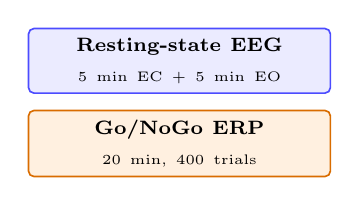
\begin{tikzpicture}
    % Resting EEG box
    \node[
        draw=blue!70,
        fill=blue!8,
        rounded corners=2pt,
        line width=0.6pt,
        text width=3.6cm,
        align=center,
        minimum height=0.75cm
    ] (rest) at (0,0) {
        \textbf{\scriptsize Resting-state EEG}\\[-1pt]
        {\tiny 5 min EC + 5 min EO}
    };

    % Go/NoGo box
    \node[
        draw=orange!85!black,
        fill=orange!12,
        rounded corners=2pt,
        line width=0.6pt,
        text width=3.6cm,
        align=center,
        minimum height=0.75cm
    ] (gonogo) at (0,-1.05) {
        \textbf{\scriptsize Go/NoGo ERP}\\[-1pt]
        {\tiny 20 min, 400 trials}
    };
\end{tikzpicture}

\vspace{0.10cm}

\raggedright
\begin{itemize}\itemsep1pt
    \item 103 children: 49 ADHD, 54 controls
    \item Age range: 6--10 years
    \item 19 channels, 500 Hz
    \item Resting-state EEG: eyes closed / eyes open
    \item ERP Go/NoGo task
\end{itemize}

\end{column}

\end{columns}

\end{frame}
%--------------------------------------------
\section{Proposal and Results}
%--------------------------------------------
% \subsection{EEG-GCIRNet: Gaussian Functional Connectivity}

\begin{frame}{Proposal 1: EEG-GCIRNet (Aim 1)}

{\centering
Gaussian Connectivity-Driven EEG Imaging for Deep Learning-Based MI Classification
\par}

\begin{figure}
    \centering
    \includegraphics[width=0.78\linewidth]{figures/Scheme EEG-CIRNET.pdf}
\end{figure}

{\centering
\textcolor{frameblue}{EEG-GCIRNet transforms EEG signals into connectivity-driven topographic maps and learns reconstruction and classification from a shared latent space}
\par}

\end{frame}

%--------------------------------------------
\begin{frame}{Proposal 1: Gaussian Functional Connectivity}
\scriptsize
\setlength{\abovedisplayskip}{2pt}
\setlength{\belowdisplayskip}{2pt}
\setlength{\jot}{2pt}

\begin{enumerate}
\setlength{\itemsep}{0.10cm}

%------------------------------------------------
\item \textbf{Band-limited EEG signal} 
{\scriptsize \cite{cohen2014analyzing}:}

\vspace{0.5cm}

For each EEG channel $x_c \in \mathbb{R}^{T}$ and frequency band $\Omega_b$

\begin{align*}
x_c^{(\Omega_b)}
&=
\mathcal{F}^{-1}
\left\{
\mathcal{F}\{x_c\};\Omega_b
\right\}.
\end{align*}

%------------------------------------------------
\item \textbf{Gaussian similarity between two EEG channels} 
{\scriptsize \cite{scholkopf2002learning}:}

\vspace{0.5cm}

where $x_c^{(\Omega_b)}$ and $x_{c'}^{(\Omega_b)}$ denote the band-filtered EEG signals 
from channels $c$ and $c'$, respectively

\begin{align*}
\kappa_G
\left(
x_c^{(\Omega_b)},x_{c'}^{(\Omega_b)};
\sigma_{\Omega_b}
\right)
&=
\exp\left(
-
\frac{
\left\|
x_c^{(\Omega_b)}-x_{c'}^{(\Omega_b)}
\right\|_2^2
}{
2\sigma_{\Omega_b}^2
}
\right)
\end{align*}

%------------------------------------------------
\vspace{0.05cm}

\begin{block}{{Gaussian Functional Connectivity matrix} 
{\scriptsize \cite{garciamurillo2023kcsfcnet}:} 
{\scriptsize \cite{garciamurillo2023kcsfcnet}:}}
\begin{align*}
K_{cc'}^{(\Omega_b)}
&=
\kappa_G
\left(
x_c^{(\Omega_b)},x_{c'}^{(\Omega_b)};
\sigma_{\Omega_b}
\right),
\qquad
\mathbf{K}^{(\Omega_b)} \in [0,1]^{C \times C}
\end{align*}
\end{block}

\end{enumerate}

\vspace{0.05cm}

{\centering
\footnotesize
\textcolor{frameblue}{
The Gaussian kernel converts spectral similarity between EEG channels into a functional connectivity matrix
}
\par}

\end{frame}

%--------------------------------------------

%==================================================
\begin{frame}{Proposal 1: Connectivity-Driven Topographic Imaging}
\scriptsize
\setlength{\abovedisplayskip}{2pt}
\setlength{\belowdisplayskip}{2pt}
\setlength{\jot}{1pt}

\begin{enumerate}
    \setlength{\itemsep}{0.08cm}

    \item \textbf{Channel-wise Gaussian Connectivity (GC) flow}
    {\scriptsize \cite{garciamurillo2023kcsfcnet}}

    $g_c^{(\Omega_b)}$ summarizes the average Gaussian connectivity of channel $c$ with all other channels.

    \begin{align*}
    g_c^{(\Omega_b)}
    &=
    \frac{1}{C}
    \sum_{\substack{c'=1 \\ c'\neq c}}^{C}
    K_{cc'}^{(\Omega_b)}
    \end{align*}

    \item \textbf{Electrode coordinates}
    {\scriptsize \cite{jasper1958ten}}

    Each normalized GC value is mapped onto its electrode position.

    \begin{align*}
    P
    &=
    \{(p_{c,x},p_{c,y})\}_{c=1}^{C},
    \qquad
    \tilde{g}_c^{(\Omega_b)}
    \rightarrow
    (p_{c,x},p_{c,y})
    \end{align*}

    \item \textbf{Barycentric interpolation}
    {\scriptsize \cite{bashivan2015learning}}

    Grid values are interpolated from neighboring electrode values.

    \begin{align*}
    V(x,y)
    &=
    \sum_{j=1}^{3}
    \lambda_j(x,y)\,v(p_j),
    \qquad
    \sum_{j=1}^{3}\lambda_j
    =
    1,
    \quad
    \lambda_j \geq 0
    \end{align*}


{\scriptsize
$V(x,y)$ is the value at point $(x,y)$, where $\lambda_j(x,y)$ are barycentric weights and $p_j$ denotes the neighboring electrode positions.
}


\end{enumerate}

\end{frame}

%==================================================
\begin{frame}{Proposal 1: Multi-band Topographic EEG Image}
\scriptsize
\setlength{\abovedisplayskip}{2pt}
\setlength{\belowdisplayskip}{2pt}
\setlength{\jot}{1pt}

    \setcounter{enumi}{3}

    \begin{block}{Multi-band topographic EEG image}
    {\scriptsize \cite{bashivan2015learning}}

    Band-specific topomaps are stacked as EEG image channels

    \begin{center}
    $
    \begin{aligned}
    Y
    &=
    \left[
    T^{(\Omega_1)},T^{(\Omega_2)},\ldots,T^{(\Omega_B)}
    \right]
    \quad
    &\in
    \mathbb{R}^{\tilde{H}\times\tilde{W}\times B}
    \end{aligned}
    $
    \end{center}

\end{block}

{\scriptsize
$\tilde{H}\times\tilde{W}$: interpolated topographic grid size; 
$B$: number of frequency bands}

\begin{figure}
    \centering
    \includegraphics[width=0.2\linewidth]{figures/topo.pdf}
\end{figure}

\begin{center}
\textcolor{frameblue}{
{The final representation preserves spatial electrode information and frequency-specific connectivity patterns}
}
\end{center}

\end{frame}

% %------------------------------------------

\begin{frame}{Proposal 1: VAE Latent Representation}
\scriptsize
\setlength{\abovedisplayskip}{2pt}
\setlength{\belowdisplayskip}{2pt}
\setlength{\jot}{2pt}

\begin{enumerate}

    \item \textbf{Encoder and latent distribution}
    {\scriptsize \cite{kingma2014autoencoding}}

    \begin{align*}
    h_E
    &=
    (f_5\circ f_4\circ f_3\circ f_2\circ f_1)(Y)
    \end{align*}

    \begin{align*}
    \mu
    &=
    W_{\mu}h_E+b_{\mu},
    \qquad
    \log\sigma^2
    =
    W_{\sigma}h_E+b_{\sigma}
    \end{align*}


    \item \textbf{Reparameterization trick}
    {\scriptsize \cite{kingma2014autoencoding}}

    \begin{align*}
    z_i
    &=
    \mu_i+
    \exp\left(
    \frac{1}{2}\log\sigma_i^2
    \right)
    \odot \epsilon_i,
    \qquad
    \epsilon_i\sim\mathcal{N}(0,I)
    \end{align*}

    \item \textbf{Shared latent representation for reconstruction and classification}

    \begin{align*}
    \hat{Y}
    &=
    D_{\theta}(z),
    \qquad
    \hat{p}
    =
    C_{\psi}(z)
    \end{align*}

\end{enumerate}

{\scriptsize
\textbf{Notation:} $Y$ is the multi-band EEG image; $f_1,\ldots,f_5$ are encoder layers; $h_E$ is the encoder output; $W_{\mu},W_{\sigma},b_{\mu},b_{\sigma}$ are learnable parameters; $\mu$ and $\log\sigma^2$ are the latent mean and log-variance; $\epsilon_i$ is Gaussian noise; $z$ is the sampled latent vector; $\hat{Y}$ is the reconstructed image; and $\hat{\mathbf{p}}$ is the predicted class-probability vector. }

\end{frame}

%--------------------------------------------
\begin{frame}{Proposal 1: Composite VAE Objective}
\scriptsize
\setlength{\abovedisplayskip}{2pt}
\setlength{\belowdisplayskip}{2pt}
\setlength{\jot}{2pt}

\begin{block}{Composite optimization objective}

\begin{align*}
\mathcal{L}_{total}
&=
\lambda_{REC}\mathcal{L}_{REC}
+
\lambda_{CLA}\mathcal{L}_{CLA}
+
\lambda_{REG}\mathcal{L}_{REG}
\end{align*}

\end{block}


\begin{enumerate}
\setlength{\itemsep}{0.08cm}

\item \textbf{Normalized reconstruction loss}

\begin{align*}
\mathcal{L}_{REC}
&=
\frac{
\frac{1}{N}
\sum_{i=1}^{N}
\left\|
Y_i-\hat{Y}_i
\right\|_F^2
}{
\frac{1}{N}
\sum_{i=1}^{N}
\left\|
Y_i-\bar{Y}
\right\|_F^2
}
\end{align*}

\item \textbf{Normalized classification loss}

\begin{align*}
\mathcal{L}_{CLA}
&=
\frac{1}{N}
\sum_{i=1}^{N}
\frac{
\mathcal{L}_{\mathrm{cce}}
\left(
\mathbf{y}_i,\hat{\mathbf{p}}_i
\right)
}{
\mathcal{L}_{\mathrm{cce}}
\left(
[0.5,0.5],\hat{\mathbf{p}}_i
\right)
}
\end{align*}

\item \textbf{Normalized latent regularization}

\begin{align*}
\mathcal{L}_{REG}
&=
\frac{1}{N\log N}
\sum_{i=1}^{N}
D_{KL}
\left(
q_{\phi}(z_i\mid Y_i)
\parallel
\mathcal{N}(0,I)
\right)
\end{align*}

\end{enumerate}

{\scriptsize
\textbf{Notation:} $\bar{Y}$ is the mean EEG image,
$\mathbf{y}_i$ is the true one-hot label,
$q_{\phi}(z_i\mid Y_i)$ is the encoder posterior,}

\end{frame}

%--------------------------------------------

\begin{frame}{Experimental Set-up EEG-GCIRNet}

\setlength{\leftmargini}{1.4em}
\setlength{\leftmarginii}{1.2em}
\setlength{\fboxsep}{1.2pt}

\vspace{0.35cm}

%==================================================
% 1. EEG-GCIRNET TRAINING
%==================================================
\noindent
\colorbox{frameblue}{\textcolor{white}{\textbf{\scriptsize 1}}}
\hspace{0.12cm}
\textbf{\normalsize Training:}

\vspace{0.04cm}

\begin{itemize}\itemsep2pt

    \item Validation: 5-fold cross-validation with an 80/20 split per subject
    \item Training: Adam optimizer, batch size $=64$, 200 epochs
    \item {Regularization:} early stopping with patience of 10 epochs based on validation loss
    \item {Hyperparameter search:} Optuna-based Bayesian optimization ($\lambda_{\mathrm{REC}}$, $\lambda_{\mathrm{CLA}}$, and $\lambda_{\mathrm{REG}}$)

\end{itemize}

\vspace{0.12cm}

%==================================================
% 2. BASELINE COMPARISON
%==================================================
\noindent \colorbox{frameblue}{\textcolor{white}{\textbf{\scriptsize 2}}} \hspace{0.12cm} {\normalsize Baseline Comparison:} \vspace{0.04cm} \begin{itemize}\itemsep2pt \item {Classical baseline:} CSP~\cite{ang2008filter}
\item {Deep learning baselines:} EEGNet~\cite{lawhern2018eegnet}, ShallowConvNet~\cite{Kim2022}, DeepConvNet~\cite{schirrmeister2017deep} 
\item {Connectivity-based baselines:} KCS-FCNet~\cite{diagnostics13061122}, KREEGNet~\cite{tobon2023kreegnet}, TCFusionNet~\cite{Musallam2021} \end{itemize} \vspace{0.12cm}

\end{frame}
% %--------------------------------------------

\begin{frame}{Results Proposal 1}

\centering Inter-subject accuracy comparison across MI classification models

\vspace{0.08cm}

\definecolor{modelBlue}{RGB}{31,119,180}
\definecolor{modelOrange}{RGB}{255,127,14}
\definecolor{modelGreen}{RGB}{44,160,44}
\definecolor{modelRed}{RGB}{214,39,40}
\definecolor{modelPurple}{RGB}{148,103,189}
\definecolor{modelBrown}{RGB}{140,86,75}
\definecolor{modelGray}{RGB}{127,127,127}
\definecolor{modelOlive}{RGB}{57, 255, 20}

\pgfplotsset{
  every axis plot/.style={solid, mark=none},
  myaxis/.style={
    width=0.8\linewidth,
    height=0.48\textheight,
    scale only axis,
    ymin=0.40, ymax=1.00,
    xmin=-0.5, xmax=49.5,
    xtick=data,
    xtick pos=bottom,
    ytick pos=left,
    tick align=inside,
    ytick={0.40,0.50,0.60,0.70,0.80,0.90,1.00},
    yticklabels={40,50,60,70,80,90,100},
    ylabel={Accuracy (\%)},
    xlabel={Subjects},
    xticklabel style={rotate=90, anchor=east, font=\tiny},
    yticklabel style={font=\tiny},
    label style={font=\scriptsize},
    axis lines=box,
    xmajorgrids,
    ymajorgrids,
    grid style={black!15},
    legend style={
        at={(0.01,0.02)},
        anchor=south west,
        draw=black!25,
        fill=white,
        fill opacity=0.85,
        text opacity=1,
        font=\tiny,
        inner sep=1pt,
        row sep=0.5pt,
        column sep=1.5pt
    },
    legend image post style={xscale=0.35},
    legend cell align=left,
    legend columns=2,
  }
}

\centering
\begin{tikzpicture}
\begin{axis}[myaxis,
  xticklabels={43,14,3,50,48,4,35,13,23,41,1,49,37,26,5,44,6,47,28,36,12,39,46,10,20,22,31,18,52,25,21,40,24,27,30,51,42,9,16,38,11,19,33,2,17,15,45,32,7,8}
]

\path[fill=red!40,    opacity=0.35] (axis cs:-0.5,0.40) rectangle (axis cs:49.5,0.60);
\path[fill=yellow!50, opacity=0.35] (axis cs:-0.5,0.60) rectangle (axis cs:49.5,0.80);
\path[fill=green!40,  opacity=0.35] (axis cs:-0.5,0.80) rectangle (axis cs:49.5,1.00);

\addplot[line width=0.9pt, color=modelBlue]
coordinates {(0,0.99500) (1,0.97000) (2,0.93500) (3,0.92500) (4,0.92500) (5,0.91000) (6,0.88000) (7,0.84000) (8,0.84000) (9,0.83000) (10,0.81000) (11,0.78970) (12,0.77000) (13,0.76500) (14,0.76500) (15,0.76000) (16,0.75560) (17,0.74870) (18,0.74500) (19,0.73850) (20,0.72570) (21,0.71000) (22,0.69170) (23,0.68000) (24,0.64710) (25,0.64000) (26,0.63000) (27,0.62000) (28,0.61500) (29,0.60500) (30,0.59000) (31,0.58000) (32,0.57500) (33,0.56220) (34,0.56000) (35,0.55900) (36,0.55500) (37,0.55000) (38,0.55000) (39,0.54870) (40,0.54500) (41,0.54480) (42,0.54000) (43,0.54000) (44,0.53500) (45,0.53330) (46,0.53000) (47,0.52000) (48,0.51670) (49,0.50000)};
\addlegendentry{EEGNet}

\addplot[line width=0.9pt, color=modelOrange]
coordinates {(0,0.98500) (1,0.97500) (2,0.98000) (3,0.97000) (4,0.96500) (5,0.96000) (6,0.87000) (7,0.94000) (8,0.93000) (9,0.94500) (10,0.88500) (11,0.83080) (12,0.84500) (13,0.89500) (14,0.88500) (15,0.90000) (16,0.85000) (17,0.81540) (18,0.83500) (19,0.74870) (20,0.79430) (21,0.78500) (22,0.80420) (23,0.85000) (24,0.74120) (25,0.77000) (26,0.79000) (27,0.73500) (28,0.69500) (29,0.85500) (30,0.82500) (31,0.58500) (32,0.76000) (33,0.58920) (34,0.61600) (35,0.61540) (36,0.70500) (37,0.68750) (38,0.56500) (39,0.54870) (40,0.64000) (41,0.64140) (42,0.58000) (43,0.54500) (44,0.58500) (45,0.88210) (46,0.64500) (47,0.58000) (48,0.60000) (49,0.63500)};
\addlegendentry{KREEGNet}

\addplot[line width=0.9pt, color=modelGreen]
coordinates {(0,0.96500) (1,0.96000) (2,0.92500) (3,0.85500) (4,0.90500) (5,0.91500) (6,0.82000) (7,0.80000) (8,0.88500) (9,0.87500) (10,0.73500) (11,0.83590) (12,0.79000) (13,0.79500) (14,0.81000) (15,0.83000) (16,0.77780) (17,0.69740) (18,0.74000) (19,0.70770) (20,0.69140) (21,0.77500) (22,0.78330) (23,0.75000) (24,0.72940) (25,0.68000) (26,0.84000) (27,0.76000) (28,0.73000) (29,0.65000) (30,0.76500) (31,0.64000) (32,0.72000) (33,0.46490) (34,0.69600) (35,0.51790) (36,0.77000) (37,0.71250) (38,0.48000) (39,0.54360) (40,0.52000) (41,0.62070) (42,0.62500) (43,0.56000) (44,0.54000) (45,0.80000) (46,0.61000) (47,0.60000) (48,0.61670) (49,0.57000)};
\addlegendentry{KCS-FCNet}

\addplot[line width=0.9pt, color=modelRed]
coordinates {(0,0.98500) (1,0.95000) (2,0.81500) (3,0.86500) (4,0.79500) (5,0.80000) (6,0.85000) (7,0.90000) (8,0.72500) (9,0.65000) (10,0.78500) (11,0.72310) (12,0.80500) (13,0.78500) (14,0.67500) (15,0.87500) (16,0.73330) (17,0.77440) (18,0.69000) (19,0.69230) (20,0.66290) (21,0.75500) (22,0.75830) (23,0.61000) (24,0.71760) (25,0.61500) (26,0.54500) (27,0.62500) (28,0.52500) (29,0.60000) (30,0.59000) (31,0.54500) (32,0.63000) (33,0.54590) (34,0.52800) (35,0.58970) (36,0.55000) (37,0.57080) (38,0.54000) (39,0.53850) (40,0.49000) (41,0.50340) (42,0.55500) (43,0.53500) (44,0.53500) (45,0.50260) (46,0.55500) (47,0.55500) (48,0.56670) (49,0.56000)};
\addlegendentry{DeepConvNet}

\addplot[line width=0.9pt, color=modelPurple]
coordinates {(0,0.98000) (1,0.96500) (2,0.96000) (3,0.96000) (4,0.94500) (5,0.93500) (6,0.86500) (7,0.90500) (8,0.87500) (9,0.92500) (10,0.89500) (11,0.86670) (12,0.85500) (13,0.86500) (14,0.91000) (15,0.92000) (16,0.83330) (17,0.83080) (18,0.75000) (19,0.70770) (20,0.73710) (21,0.79000) (22,0.80420) (23,0.75000) (24,0.71760) (25,0.69500) (26,0.74000) (27,0.62000) (28,0.70500) (29,0.68500) (30,0.58500) (31,0.61500) (32,0.75000) (33,0.60540) (34,0.58400) (35,0.55380) (36,0.62000) (37,0.70830) (38,0.54500) (39,0.62560) (40,0.63000) (41,0.55170) (42,0.62000) (43,0.59500) (44,0.53000) (45,0.67690) (46,0.63000) (47,0.63000) (48,0.59170) (49,0.64000)};
\addlegendentry{ShallowConvNet}

\addplot[line width=0.9pt, color=modelBrown]
coordinates {(0,0.99000) (1,0.97500) (2,0.94000) (3,0.88500) (4,0.95000) (5,0.90500) (6,0.85000) (7,0.81500) (8,0.83500) (9,0.84000) (10,0.79500) (11,0.86150) (12,0.79500) (13,0.82500) (14,0.80000) (15,0.83500) (16,0.82780) (17,0.72310) (18,0.86500) (19,0.67180) (20,0.68570) (21,0.71000) (22,0.81670) (23,0.72000) (24,0.72940) (25,0.70500) (26,0.73000) (27,0.68500) (28,0.75500) (29,0.75500) (30,0.79500) (31,0.60000) (32,0.72500) (33,0.62160) (34,0.54400) (35,0.58970) (36,0.66500) (37,0.66250) (38,0.55500) (39,0.58970) (40,0.53000) (41,0.61380) (42,0.61000) (43,0.52500) (44,0.47000) (45,0.71280) (46,0.59500) (47,0.57500) (48,0.58750) (49,0.56000)};
\addlegendentry{TCFusionNet}

\addplot[line width=0.9pt, color=modelGray]
coordinates {(0,0.98100) (1,0.97100) (2,0.95400) (3,0.87800) (4,0.89100) (5,0.85000) (6,0.78300) (7,0.83600) (8,0.86000) (9,0.89300) (10,0.72500) (11,0.77500) (12,0.70200) (13,0.82900) (14,0.73300) (15,0.78700) (16,0.69500) (17,0.65200) (18,0.61200) (19,0.66200) (20,0.64400) (21,0.66600) (22,0.85300) (23,0.66300) (24,0.65800) (25,0.68300) (26,0.64400) (27,0.58000) (28,0.65100) (29,0.60600) (30,0.68600) (31,0.49000) (32,0.59200) (33,0.49200) (34,0.56100) (35,0.51800) (36,0.54800) (37,0.58300) (38,0.53300) (39,0.52400) (40,0.58300) (41,0.57900) (42,0.58100) (43,0.59700) (44,0.50400) (45,0.64200) (46,0.51100) (47,0.51400) (48,0.53900) (49,0.54200)};
\addlegendentry{CSP}

\addplot[line width=1.2pt, color=modelOlive]
coordinates {(0,0.94000) (1,0.95490) (2,0.91500) (3,0.84500) (4,0.95000) (5,0.95000) (6,0.82000) (7,0.86990) (8,0.89000) (9,0.80000) (10,0.73000) (11,0.90250) (12,0.85000) (13,0.88500) (14,0.84500) (15,0.90500) (16,0.76700) (17,0.90250) (18,0.86500) (19,0.86150) (20,0.72000) (21,0.78490) (22,0.88750) (23,0.86490) (24,0.83500) (25,0.82500) (26,0.84000) (27,0.84500) (28,0.80490) (29,0.81500) (30,0.84000) (31,0.80000) (32,0.83000) (33,0.62100) (34,0.81600) (35,0.74350) (36,0.86000) (37,0.83750) (38,0.75990) (39,0.67690) (40,0.75500) (41,0.71700) (42,0.76000) (43,0.76000) (44,0.69500) (45,0.80000) (46,0.67990) (47,0.63500) (48,0.88800) (49,0.76500)};
\addlegendentry{EEG-GCIRNet}

\end{axis}
\end{tikzpicture}

\vspace{0.08cm}

{\centering
\textcolor{frameblue}{Subjects are sorted according to EEGNet accuracy; background colors indicate Bad ($\leq$60\%), Mid (60--80\%), and Good ($>$80\%) performance groups}
\par}

\end{frame}

%--------------------------------------------
\begin{frame}{Results Proposal 1: Loss-Weight Analysis}

\centering Distribution of learned weights for reconstruction, classification, and latent regularization

\vspace{0.08cm}

\centering
\includegraphics[width=0.52\linewidth]{figures/distributions_histogram_mid_good_with_mode.pdf}

\vspace{0.08cm}

{\centering
\textcolor{frameblue}{The learned weights show how the model balances reconstruction, classification, and latent-space regularization across performance groups}
\par}

\end{frame}

%--------------------------------------------
\begin{frame}{Results Proposal 1: Visual Reconstruction}

\vspace{0.08cm}

\centering Connectivity-driven topographic reconstructions for representative subjects

{\centering
\includegraphics[width=\linewidth]{figures/topomaps_bands_14.pdf}

{\scriptsize (a) Subject 14 -- Good group}

\vspace{0.12cm}

\par}

{\centering
\textcolor{frameblue}{The reconstructed maps allow visual inspection of the spatial--spectral\\ patterns learned by the model}
\par}

\end{frame}
%--------------------------------------------

%--------------------------------------------
% \begin{frame}{Results Proposal 1: Group-wise Accuracy Gain}

% \centering Accuracy gain according to subject performance groups

% \vspace{0.12cm}

% \centering
% \renewcommand{\arraystretch}{1.18}

% \begin{tabular}{llcc}
% \toprule
% \textbf{Approach} & \textbf{Group} & \textbf{Accuracy [\%]} & \textbf{Gain [\%]} \\
% \midrule
% \multirow{3}{*}{EEGNet}
% & Good & 89.64 & -- \\
% & Mid  & 70.54 & -- \\
% & Bad  & 54.65 & -- \\
% \midrule
% \multirow{3}{*}{\textbf{EEG-GCIRNet (Ours)}}
% & Good & 87.86 & $-1.78$ \\
% & Mid  & \textbf{84.24} & $\mathbf{13.70}$ \\
% & Bad  & \textbf{76.20} & $\mathbf{21.55}$ \\
% \bottomrule
% \end{tabular}

% \vspace{0.20cm}

% {\centering
% \textcolor{frameblue}{The largest improvements were obtained for Mid and Bad subjects, suggesting better robustness in challenging cases}
% \par}

% \end{frame}
%--------------------------------------------

%--------------------------------------------
\begin{frame}{Results Proposal 1: Hypothesis Testing}

\centering Average rankings and statistical comparison across models

\vspace{0.12cm}

\centering
\renewcommand{\arraystretch}{1.18}

\begin{tabular}{lcc}
\toprule
\textbf{Model} & \textbf{Avg. Ranking} & \textbf{Avg. T-Test \emph{p}-Value} \\
\midrule
CSP & $6.30$ & $0.23$ \\
EEGNet & $5.76$ & $0.22$ \\
KCS-FCNet & $4.58$ & $0.25$ \\
KREEGNet & $2.48$ & $0.07$ \\
DeepConvNet & $6.42$ & $0.17$ \\
ShallowConvNet & $3.40$ & $0.19$ \\
TCFusionNet & $4.34$ & $0.26$ \\
\textbf{EEG-GCIRNet (Ours)} & $\mathbf{2.32}$ & $\mathbf{0.007}$ \\
\bottomrule
\end{tabular}

\vspace{0.20cm}

{\centering
\textcolor{frameblue}{EEG-GCIRNet obtained the best average ranking and the lowest average \emph{p}-value, supporting its consistent performance advantage}
\par}

\end{frame}
%--------------------------------------------
% \subsection{TEKTE-Net: Takens-Based Kernel Transfer Entropy}

\begin{frame}{Proposal 2: TEKTE-Net (Aim 2)}

\centering Takens-based Kernel TE Connectivity Network for
MI Classification

\vspace{0.15cm}

\begin{figure}
    \centering
    \includegraphics[width=\linewidth]{figures/Metodology.pdf}
\end{figure}

\vspace{-0.1cm}

\begin{center}
\textcolor{frameblue}{TEKTE-Net combines Takens state-space reconstruction and kernel Transfer Entropy to model nonlinear, time-delayed, and directed predictive dependencies among EEG channels}
\end{center}

\end{frame}

%--------------------------------------------
\begin{frame}{Proposal 2: Nonlinear Filtering and Takens Embedding}
\scriptsize
\setlength{\abovedisplayskip}{2pt}
\setlength{\belowdisplayskip}{2pt}
\setlength{\jot}{2pt}

\begin{enumerate}
\setlength{\itemsep}{0.08cm}

%------------------------------------------------
\item \textbf{Nonlinear filtering}
{\scriptsize \cite{schirrmeister2017deep}}

The multichannel EEG input $\mathbf{X}$ is transformed into nonlinearly filtered channels:

\begin{align*}
\boldsymbol{\Phi}
&=
\varphi(\mathbf{X}\mid \theta),
\qquad
\boldsymbol{\Phi}
=
\left[
\varphi(\mathbf{x}_c\mid \theta_c)
\right]_{c=1}^{C}
\in
\mathbb{R}^{T_{\phi}\times C}
\end{align*}

%------------------------------------------------
\item \textbf{Takens embedding operator}
{\scriptsize \cite{takens1981detecting}}

A non-trainable convolutional embedding kernel stacks present, past, and delayed states:

\begin{align*}
\mathbf{W}
&=
\left[
\mathbf{W}_{\tau,1,0}
\mid
\mathbf{W}_{\tau,D',1}
\mid
\mathbf{W}_{\tau,D,\mu}
\right]
\end{align*}

%------------------------------------------------
\item \textbf{Takens embedded tensor}

\begin{align*}
\mathbf{Z}
&=
\mathbf{W}*\boldsymbol{\Phi},
\qquad
\mathbf{Z}
=
\left[
\mathbf{Z}_c
\right]_{c=1}^{C}
\in
\mathbb{R}^{T_z\times(D+D'+1)\times C}
\end{align*}
\vspace{-0.35cm}

\end{enumerate}

\vspace{0.04cm}

{\scriptsize
\textbf{Notation:}
$\mathbf{X}\in\mathbb{R}^{T\times C}$ is the multichannel EEG input;
$\boldsymbol{\Phi}$ denotes the nonlinearly filtered EEG representation;
$\mathbf{W}$ is the fixed Takens embedding kernel;
$\tau$ is the time delay;
$D$ and $D'$ are embedding dimensions;
$\mu$ is the interaction delay;
and $\mathbf{Z}$ is the embedded tensor used for TE estimation
}

 \end{frame}
%--------------------------------------------

\begin{frame}{Proposal 2: Kernel Entropy and Rational Quadratic Similarity}
\scriptsize
\setlength{\abovedisplayskip}{2pt}
\setlength{\belowdisplayskip}{2pt}
\setlength{\jot}{2pt}

\begin{enumerate}
\setlength{\itemsep}{0.08cm}

%------------------------------------------------
\item \textbf{Kernel entropy approximation}
{\scriptsize \cite{giraldo2015measures}.}

\begin{align*}
H\{\mathbf{v}\}
&\approx
S(\mathbf{K}_{\mathbf{v}})
=
\log
\left(
\operatorname{tr}
\left(
\mathbf{K}_{\mathbf{v}}
\right)
\right)
\end{align*}

\begin{align*}
H\{\mathbf{v},\mathbf{v}'\}
&\approx
S\left(
\frac{
\mathbf{K}_{\mathbf{v}}
\circ
\mathbf{K}_{\mathbf{v}'}
}{
\operatorname{tr}
\left(
\mathbf{K}_{\mathbf{v}}
\circ
\mathbf{K}_{\mathbf{v}'}
\right)
}
\right)
\end{align*}

%------------------------------------------------
\item \textbf{Kernel matrices for TE estimation}

\begin{align*}
\mathbf{K}_{c'0}
&=
\left[
\kappa
\left(
z_{c't},
z_{c's}
\mid
\ell_{c'0}
\right)
\right]_{t,s=1}^{T_z}
\end{align*}

\begin{align*}
\mathbf{K}_{c'1}
&=
\left[
\kappa
\left(
\mathbf{z}_{c't-1},
\mathbf{z}_{c's-1}
\mid
\ell_{c'1}
\right)
\right]_{t,s=1}^{T_z},
\qquad
\mathbf{K}_{c\mu}
=
\left[
\kappa
\left(
\mathbf{z}_{ct-\mu},
\mathbf{z}_{cs-\mu}
\mid
\ell_{c\mu}
\right)
\right]_{t,s=1}^{T_z}
\end{align*}

%------------------------------------------------

\begin{block}{Rational Quadratic (RQ) kernel {\scriptsize \cite{rasmussen2006gaussian}.}}

\begin{align*}
\kappa(\mathbf{z},\mathbf{z}')
&=
\left(
1+
\frac{1}{2\alpha}
\left\|
\mathbf{z}-\mathbf{z}'
\right\|_{\mathbf{A}}^2
\right)^{-\alpha}
\end{align*}

\end{block}

\end{enumerate}

% {\fontsize{7.2}{8}\selectfont
% \textbf{Notation:}
% $\mathbf{v}$ and $\mathbf{v}'$ denote embedded random variables;
% $\mathbf{K}_{\mathbf{v}}$ is the kernel similarity matrix;
% $\circ$ denotes the Hadamard product;
% $\operatorname{tr}(\cdot)$ is the matrix trace;
% $\kappa(\cdot,\cdot)$ is the RQ kernel;
% $\ell$ is the kernel length-scale;
% $T_z$ is the number of embedded samples;
% $\alpha$ controls the RQ kernel shape; and
% $\mathbf{A}$ defines the weighted distance metric.
% }




\end{frame}
%--------------------------------------------
\begin{frame}{Information-Theoretic Connectivity: Entropy and Mutual Information}

\scriptsize
\setlength{\abovedisplayskip}{3pt}
\setlength{\belowdisplayskip}{3pt}
\setlength{\jot}{2pt}

\begin{columns}[T,totalwidth=\textwidth]

%==================================================
% LEFT COLUMN
%==================================================
\begin{column}{0.54\textwidth}

\begin{enumerate}
\setlength{\itemsep}{0.16cm}

\item \textbf{Shannon entropy}
{\scriptsize \cite{shannon1948mathematical}}

\[
H(X)=-\int_{\mathcal{X}} g(x)\log g(x)\,dx
\]

\item \textbf{Rényi entropy}
{\scriptsize \cite{renyi1961measures}}

\[
H_{\alpha}(X)=
\frac{1}{1-\alpha}
\log\!\left(
\int_{\mathcal{X}} g(x)^{\alpha}\,dx
\right),
\qquad
\alpha>0,\ \alpha\neq 1
\]

\item \textbf{Mutual information}
{\scriptsize \cite{cover2006elements}}

\[
I(X;Y)=H(X)+H(Y)-H(X,Y)
\]

\end{enumerate}

\end{column}

%==================================================
% RIGHT COLUMN
%==================================================
\begin{column}{0.42\textwidth}
\centering

\resizebox{0.7\linewidth}{!}{%
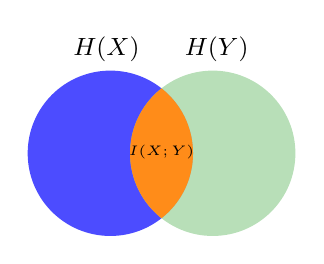
\begin{tikzpicture}
    \fill[blue!70] (0,0) circle (1.05);
    \fill[green!55!black!35, opacity=0.80] (1.30,0) circle (1.05);

    \begin{scope}
        \clip (0,0) circle (1.05);
        \fill[orange!90] (1.30,0) circle (1.05);
    \end{scope}

    \node[font=\bfseries\small] at (-0.05,1.32) {$H(X)$};
    \node[font=\bfseries\small] at (1.35,1.32) {$H(Y)$};
    \node[font=\bfseries\fontsize{5}{6}\selectfont] at (0.65,0.02) {$I(X;Y)$};
\end{tikzpicture}%
}

\end{column}

\end{columns}

\vspace{0.22cm}

{\scriptsize
\textbf{Notation:}
$X$ and $Y$ are random variables;
$g(x)$ is the probability density of $X$;
$\mathcal{X}$ is the support of $X$;
$\alpha$ is the Rényi order;
$H(X,Y)$ is the joint entropy; and
$I(X;Y)$ is the shared information between $X$ and $Y$.
}

\vspace{0.30cm}

{\centering
\color{frameblue}\footnotesize
Shannon entropy quantifies uncertainty, Rényi entropy generalizes it, and mutual information measures shared information, but it remains symmetric and does not indicate directionality.
\par}

\end{frame}


%--------------------------------------------

\begin{frame}{Information-Theoretic Connectivity: From Mutual Information to TE}

\scriptsize
\setlength{\abovedisplayskip}{2pt}
\setlength{\belowdisplayskip}{2pt}
\setlength{\jot}{2pt}

\begin{enumerate}
\setcounter{enumi}{3}

\item \textbf{Transfer Entropy as Conditional Mutual Information}
{\scriptsize \cite{schreiber2000measuring}}

\[
TE(c\rightarrow c')
=
I\left(
\ve{z}_{c,t-\mu};
z_{c',t}
\mid
\ve{z}_{c',t-1}
\right)
\]

\vspace{0.04cm}

\[
\begin{aligned}
TE(c\rightarrow c')
=&\;
H_S\{z_{c',t},\ve{z}_{c',t-1}\}
+
H_S\{\ve{z}_{c',t-1},\ve{z}_{c,t-\mu}\}\\
&-
H_S\{\ve{z}_{c',t-1}\}
-
H_S\{z_{c',t},\ve{z}_{c',t-1},\ve{z}_{c,t-\mu}\}
\end{aligned}
\]

\end{enumerate}

\vspace{0.10cm}

\begin{center}
\begin{minipage}{0.18\textwidth}
\centering
\resizebox{1.45cm}{!}{\input{figures/venn_cpcp}}

{\tiny
$H_S\{z_{c',t},\ve{z}_{c',t-1}\}$
}
\end{minipage}
\hfill
\begin{minipage}{0.18\textwidth}
\centering
\resizebox{1.45cm}{!}{\input{figures/venn_ccp}}

{\tiny
$H_S\{\ve{z}_{c',t-1},\ve{z}_{c,t-\mu}\}$
}
\end{minipage}
\hfill
\begin{minipage}{0.18\textwidth}
\centering
\resizebox{1.45cm}{!}{\input{figures/venn_cp}}

{\tiny
$H_S\{\ve{z}_{c',t-1}\}$
}
\end{minipage}
\hfill
\begin{minipage}{0.18\textwidth}
\centering
\resizebox{1.45cm}{!}{% ===== Control de saturación de los primarios (0-100) =====
\def\TONE{45} % más bajo = más claro (pastel)

% Colores pastel basados en primarios
\colorlet{softred}{red!\TONE!white}
\colorlet{softgreen}{green!\TONE!white}
\colorlet{softblue}{blue!\TONE!white}

\begin{tikzpicture}[line cap=round,line join=round]
  %--- parámetros geométricos
  \def\R{1.55}
  \def\sep{2.25}
  \def\drop{1.35}

  % Etiquetas bajo los diagramas SUPERIORES
  \pgfmathsetmacro{\UNDERPAD}{0.35}
  \pgfmathsetmacro{\yunder}{\drop + \R + \UNDERPAD}

  % Controles de la zona TE (parte inferior)
  \def\yTE{-5.6}
  \pgfmathsetmacro{\TEeqoffsetBelow}{0.9}

  \tikzset{
    outline/.style={draw=black!75,line width=0.6pt},
    lab/.style={font=\Large, text=black!85}
  }

  % posiciones fila superior
  \def\xA{-8} \def\xB{-2} \def\xC{4} \def\xD{10}

  % === (1) ===
  \begin{scope}[shift={({\xA},{0})},scale=0.5]
    \coordinate (L) at (-\sep/2,0);
    \coordinate (R) at ( \sep/2,0);
    \coordinate (B) at (0,-\drop);
    \begin{scope}[blend group=screen]
      \fill[softred,   fill opacity=0.90] (L) circle (\R);
      \fill[softgreen, fill opacity=0.90] (R) circle (\R);
      \fill[softblue,  fill opacity=0.90] (B) circle (\R);
    \end{scope}
    \draw[outline] (L) circle (\R);
    \draw[outline] (R) circle (\R);
    \draw[outline] (B) circle (\R);
    % === Etiquetas dentro de cada círculo (con desplazamientos) ===
    \node[font=\small, align=center] at ([xshift=-0.22cm,yshift= 0.26cm] L) {$\ve{z}_{ct-\mu}$};
    \node[font=\small, align=center] at ([xshift=0.18cm, yshift=0.30cm] R) {$\ve{z}_{c't-1}$};
    \node[font=\small, align=center] at ([yshift=-0.34cm] B) {$z_{c't}$};
    % =========================================
    %\node[lab, align=center] at (0,-\yunder){$\;H_S\!\bigl\{\, \ve{z}_{c't},\, \ve{z}_{c't-1},\, \ve{z}_{ct-\mu} \,\bigr\}$};
  \end{scope}
\end{tikzpicture}}

{\tiny
$H_S\{z_{c',t},\ve{z}_{c',t-1},\ve{z}_{c,t-\mu}\}$
}
\end{minipage}
\hfill
\begin{minipage}{0.18\textwidth}
\centering
\resizebox{1.45cm}{!}{% ===== Control de saturación de los primarios (0-100) =====
\def\TONE{45} % más bajo = más claro (pastel)

% Colores pastel basados en primarios
\colorlet{softred}{red!\TONE!white}
\colorlet{softgreen}{green!\TONE!white}
\colorlet{softblue}{blue!\TONE!white}

\begin{tikzpicture}[line cap=round,line join=round]
  %--- parámetros geométricos
  \def\R{1.55}
  \def\sep{2.25}
  \def\drop{1.35}

  % Etiquetas bajo los diagramas SUPERIORES
  \pgfmathsetmacro{\UNDERPAD}{0.35}
  \pgfmathsetmacro{\yunder}{\drop + \R + \UNDERPAD}

  % Controles de la zona TE (parte inferior)
  \def\yTE{-5.6}
  \pgfmathsetmacro{\TEeqoffsetBelow}{0.9}

  \tikzset{
    outline/.style={draw=black!75,line width=0.6pt},
    lab/.style={font=\Large, text=black!85}
  }

  % posiciones fila superior
  \def\xA{-8} \def\xB{-2} \def\xC{4} \def\xD{10}

  % ---- Conjunto inferior (TE)
  \pgfmathsetmacro{\xCenter}{(\xA+\xD)/2}
  \begin{scope}[scale=0.5]
    \coordinate (L) at (-\sep/2,0);
    \coordinate (R) at ( \sep/2,0);
    \coordinate (B) at (0,-\drop);
    \begin{scope}[blend group=screen]
      \begin{scope}
        \clip (B) circle (\R);
        \clip (L) circle (\R);
        \fill[softred, fill opacity=0.90, even odd rule] (-6,-7) rectangle (6,4) (R) circle (\R);
        \fill[softblue, fill opacity=0.90, even odd rule] (-6,-7) rectangle (6,4) (R) circle (\R);
      \end{scope}
    \end{scope}
    \draw[outline] (L) circle (\R);
    \draw[outline] (R) circle (\R);
    \draw[outline] (B) circle (\R);
    % Etiquetas internas (TE)
    \node[font=\small, align=center] at ([xshift=-0.22cm,yshift= 0.26cm] L) {$\ve{z}_{ct-\mu}$};
    \node[font=\small, align=center] at ([xshift=0.18cm, yshift=0.30cm] R) {$\ve{z}_{c't-1}$};
    \node[font=\small, align=center] at ([yshift=-0.34cm] B) {$z_{c't}$};
  \end{scope}


\end{tikzpicture}}

{\tiny
$\mathrm{TE}(c\rightarrow c')$
}
\end{minipage}
\end{center}

\vspace{0.08cm}

{\centering
\color{frameblue}\footnotesize
Transfer Entropy captures directional predictive information by conditioning on the target history; in TEKTE-Net, it is approximated through kernel-based Rényi entropy.
\par}

\end{frame}
%--------------------------------------------

\begin{frame}{Proposal 2: Kernel TE and Classification Model}

\scriptsize
\setlength{\abovedisplayskip}{2pt}
\setlength{\belowdisplayskip}{2pt}
\setlength{\jot}{2pt}

\begin{enumerate}
\setlength{\itemsep}{0.08cm}

%------------------------------------------------
\item \textbf{Kernel Transfer Entropy approximation}
{\scriptsize \cite{schreiber2000measuring,yu2019multivariate}}

\begin{align*}
TE_{cc'}
\approx&
-
S
\left(
\mathbf{K}_{c'0},
\mathbf{K}_{c'1},
\mathbf{K}_{c\mu}
\right)
+
S
\left(
\mathbf{K}_{c'1},
\mathbf{K}_{c\mu}
\right)
\nonumber\\
&-
S
\left(
\mathbf{K}_{c'1}
\right)
+
S
\left(
\mathbf{K}_{c'0},
\mathbf{K}_{c'1}
\right)
\end{align*}

%------------------------------------------------
\item \textbf{TE matrix from all directed channel pairs}
{\scriptsize \cite{schreiber2000measuring}}

\begin{align*}
\mathbf{TE}
&=
TE(\mathbf{Z}\mid \mathbf{A})
=
\left[
TE_{cc'}
\right]_{c,c'=1}^{C}
\in
\mathbb{R}^{C\times C}
\end{align*}

\end{enumerate}

\vspace{0.08cm}

\begin{block}{End-to-end TEKTE-Net model {\scriptsize \cite{takens1981detecting,goodfellow2016deep}}}
\centering
\begin{subequations}
\begin{align*}
\boldsymbol{\Phi}
&=
\varphi(\mathbf{X}\mid\theta)
\\
\mathbf{Z}
&=
\mathbf{W}*\boldsymbol{\Phi}
\\
\mathbf{TE}
&=
TE(\mathbf{Z}\mid\mathbf{A})
\\
p(y\mid\mathbf{X})
&=
\sigma
\left(
f
\left(
\operatorname{vec}
\left(
\mathbf{TE}
-
\operatorname{diag}(\mathbf{TE})
\right)
\mid
\vartheta
\right)
\right)
\end{align*}
\end{subequations}
\end{block}

\vspace{0.04cm}

{\centering
\footnotesize
\textcolor{frameblue}{
TEKTE-Net learns directed nonlinear EEG connectivity and maps it to the posterior class probability.
}
\par}

\end{frame}
%--------------------------------------------
\begin{frame}{Experimental Set-up TEKTE-Net: Semi-synthetic Data}

\setlength{\leftmargini}{1.4em}
\setlength{\leftmarginii}{1.2em}
\setlength{\fboxsep}{1.2pt}

\vspace{0.30cm}

%==================================================
% 1. DATA GENERATION AND LABELS
%==================================================
\noindent
\colorbox{frameblue}{\textcolor{white}{\textbf{\scriptsize 1}}}
\hspace{0.12cm}
\textbf{\normalsize Semi-synthetic Data and Labels:}

\vspace{0.04cm}

\begin{itemize}\itemsep2pt
    \item Surrogate EEG trials generated from two predefined directed structures: G1 and G2
    \item Binary labels assigned according to the interaction structure: G1 vs. G2
    \item Dataset: 1000 trials, 500 from G1 and 500 from G2
\end{itemize}

\vspace{0.10cm}

%==================================================
% 2. TRAINING
%==================================================
\noindent
\colorbox{frameblue}{\textcolor{white}{\textbf{\scriptsize 2}}}
\hspace{0.12cm}
\textbf{\normalsize Training:}

\vspace{0.04cm}

\begin{itemize}\itemsep2pt
    \item Validation: stratified 5-fold cross-validation
    \item Training: Adam optimizer, batch size $=32$, maximum 1000 epochs
    \item Regularization: early stopping with patience of 5 epochs based on validation loss
\end{itemize}

\vspace{0.10cm}

%==================================================
% 3. HYPERPARAMETER SEARCH
%==================================================
\noindent
\colorbox{frameblue}{\textcolor{white}{\textbf{\scriptsize 3}}}
\hspace{0.12cm}
\textbf{\normalsize Hyperparameter Search:}

\vspace{0.04cm}

\begin{itemize}\itemsep2pt
    \item Bayesian optimization of TEKTE-Net architectural hyperparameters
    \item Selected configuration: $D=8$, $D'=3$, $\tau=2$, $\mu=4$, $K=95$
\end{itemize}
\end{frame}

%--------------------------------------------

\begin{frame}{Results Proposal 2: Synthetic Directed Structures}

\centering
\large
Synthetic benchmarks for validating directed information flow

\vspace{0.25cm}

\begin{columns}[T,totalwidth=0.95\textwidth]

% ================= G1 =================
\begin{column}{0.48\textwidth}
\centering
\textbf{G1}

\vspace{0.15cm}

\resizebox{0.62\linewidth}{!}{
    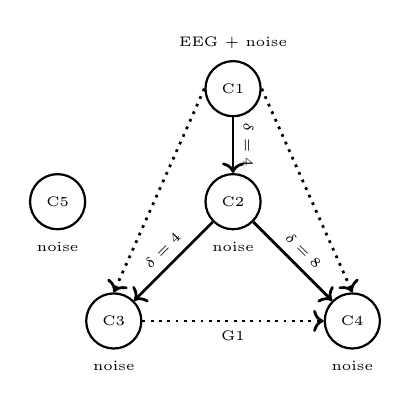
\begin{tikzpicture}[
	font=\tiny,
	every node/.style={transform shape},
	every path/.style={line width=1 pt},
	roundnode/.style={circle, draw=black, thick, minimum size=7mm},
	]
	%Nodes
	\node[roundnode] (c1) {C1};
	\node[above=0.1mm of c1] {EEG + noise};
    % \node[roundnode] (c2) [below=of c1]{C2};	
    \usetikzlibrary{positioning} % for 'below=of'
    \pgfmathsetmacro{\rsqrt}{1/sqrt(2)} % ≈ 0.70710678
    \node[roundnode] (c2) [below=\rsqrt cm of c1]{C2};


    \node[below=0.1mm of c2] {noise};
	\node[roundnode] (c3) [below left=of c2] {C3};
	\node[below=0.1mm of c3] {noise};
	\node[roundnode] (c4) [below right=of c2] {C4};
	\node[below=0.1mm of c4] {noise};
	\node[roundnode] (c5) [left=15mm of c2] {C5};
	\node[below=0.1mm of c5] {noise};
	
	
	%Lines
	\draw[->] (c1.south) -- (c2.north) node[midway, sloped, above] {$\delta = 4$};
	\draw[->] (c2.south west) -- (c3.north east) node[midway, sloped, above] {$\delta = 4$};
	\draw[->] (c2.south east) -- (c4.north west) node[midway, sloped, above] {$\delta = 8$};
	
	\draw[->, dotted] (c1.west) -- (c3.north);
	\draw[->, dotted] (c1.east) -- (c4.north);
	\draw[->, dotted] (c3.east) -- (c4.west) node[midway, sloped, below] {G1};;
	
\end{tikzpicture}
}
\end{column}

% ================= G2 =================
\begin{column}{0.48\textwidth}
\centering
\textbf{G2}

\vspace{0.15cm}

\resizebox{0.62\linewidth}{!}{
    	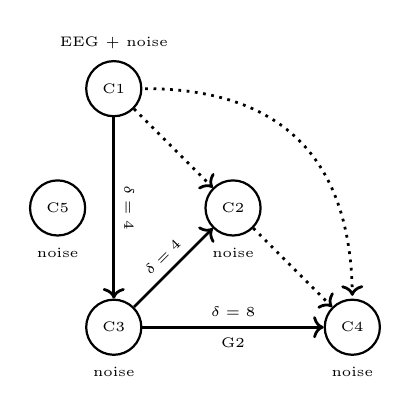
\begin{tikzpicture}[
	font=\tiny,
	every node/.style={transform shape},
	every path/.style={line width=1 pt},
	roundnode/.style={circle, draw=black, thick, minimum size=7mm},
	]
	%Nodes
	\node[roundnode] (c1) {C1};
	\node[above=0.1mm of c1] {EEG + noise};
	\node[roundnode] (c2) [below right=of c1]{C2};
	\node[below=0.1mm of c2] {noise};
	\node[roundnode] (c3) [below left=of c2] {C3};
	\node[below=0.1mm of c3] {noise};
	\node[roundnode] (c4) [below right=of c2] {C4};
	\node[below=0.1mm of c4] {noise};
	\node[roundnode] (c5) [left=15mm of c2] {C5};
	\node[below=0.1mm of c5] {noise};
	
	
	%Lines
	\draw[->] (c1.south) -- (c3.north) node[midway, sloped, above] {$\delta = 4$};
	\draw[->] (c3.north east) -- (c2.south west) node[midway, sloped, above] {$\delta = 4$};
	\draw[->] (c3.east) -- (c4.west) node[midway, sloped, above] {$\delta = 8$} node[midway, below] {G2};;
		
	\draw[->, dotted] (c1.south east) -- (c2.north west);
	\draw[->, dotted, shorten >=1pt, shorten <=1pt]	(c1.east) to[out=0, in=90, looseness=1.2] (c4.north);
	\draw[->, dotted] (c2.south east) -- (c4.north west);

	
\end{tikzpicture}
}
\end{column}

\end{columns}

\vfill

{\color{frameblue}\small
Each benchmark includes one real EEG channel, three synthetic channels, and one noise channel to evaluate whether TEKTE-Net recovers different directed interaction patterns
}

\end{frame}

\begin{frame}{Results Proposal 2: Estimated TE Matrices}

\centering
\large
Directed connectivity patterns recovered by TEKTE-Net

\vspace{0.25cm}

\begin{columns}[T,totalwidth=0.95\textwidth]

% ================= G1 =================
\begin{column}{0.48\textwidth}
\centering
\textbf{G1}

\vspace{0.65cm} % aligns G1 with G2 matrix

\resizebox{0.62\linewidth}{!}{
    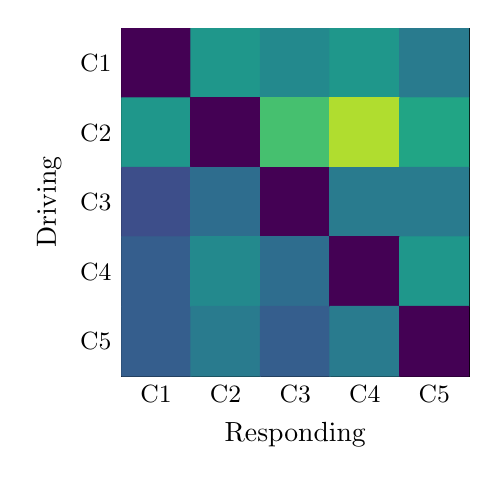
\begin{tikzpicture}
\begin{axis}[
    xlabel={Responding},
    ylabel={Driving},
    xtick={1,2,3,4,5},
    ytick={1,2,3,4,5},
    xticklabels={C1, C2, C3, C4, C5},
    yticklabels={C1, C2, C3, C4, C5},
    colormap/viridis,
    % colormap name=coolwarm,
    % colorbar,
    % colorbar style={
    % ytick={0,0.05,0.10,0.15},
    % yticklabels={0.00, 0.05, 0.10, 0.15},
    % width=0.4cm,
    % },
    point meta min=0,
    point meta max=0.17,
    enlargelimits=false,
    tick label style={font=\small},
    width=6cm,
    height=6cm,
    y dir=reverse,
]
\addplot[
    matrix plot*,
    mesh/cols=5,
    point meta=explicit,
] table [meta=C] {
x y C
1 1 0.00
2 1 0.09
3 1 0.08
4 1 0.09
5 1 0.07
1 2 0.09
2 2 0.00
3 2 0.12
4 2 0.15
5 2 0.10
1 3 0.04
2 3 0.06
3 3 0.00
4 3 0.07
5 3 0.07
1 4 0.05
2 4 0.08
3 4 0.06
4 4 0.00
5 4 0.09
1 5 0.05
2 5 0.07
3 5 0.05
4 5 0.07
5 5 0.00
};
\end{axis}
\end{tikzpicture}

}
\end{column}

% ================= G2 =================
\begin{column}{0.48\textwidth}
\centering
\textbf{G2}

\vspace{0.15cm}

\resizebox{0.70\linewidth}{!}{
    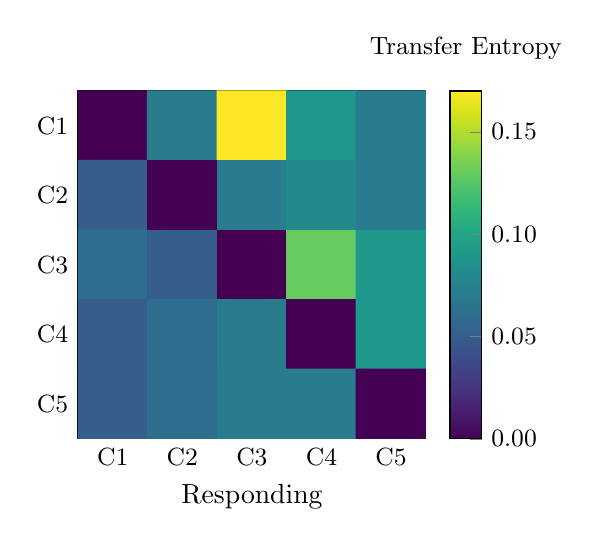
\begin{tikzpicture}
\begin{axis}[
    xlabel={Responding},
    xtick={1,2,3,4,5},
    ytick={1,2,3,4,5},
    xticklabels={C1, C2, C3, C4, C5},
    yticklabels={C1, C2, C3, C4, C5},
    colormap/viridis,
    % colormap name=coolwarm,
    colorbar,
    colorbar style={
    title={Transfer Entropy},
    title style={font=\small, yshift=2pt},
    ytick={0,0.05,0.10,0.15},
    yticklabels={0.00, 0.05, 0.10, 0.15},
    tick pos=right,
    width=0.4cm,
    yticklabel style={font=\small},
},
    point meta min=0,
    point meta max=0.17,
    enlargelimits=false,
    tick label style={font=\small},
    width=6cm,
    height=6cm,
    y dir=reverse
]
\addplot[
    matrix plot*,
    mesh/cols=5,
    point meta=explicit,
] table [meta=C] {
x y C
1 1 0.00
2 1 0.07
3 1 0.17
4 1 0.09
5 1 0.07
1 2 0.05
2 2 0.00
3 2 0.07
4 2 0.08
5 2 0.07
1 3 0.06
2 3 0.05
3 3 0.00
4 3 0.13
5 3 0.09
1 4 0.05
2 4 0.06
3 4 0.07
4 4 0.00
5 4 0.09
1 5 0.05
2 5 0.06
3 5 0.07
4 5 0.07
5 5 0.00
};
\end{axis}
\end{tikzpicture}

}
\end{column}

\end{columns}

\vfill

{\color{frameblue}\small
TEKTE-Net reached $97.0\pm1.7\%$ accuracy and recovered the main directed links in G1 and G2, although the weak/noise-sensitive $C3\!\rightarrow\!C2$ pathway was not clearly detected
}

\end{frame}

%--------------------------------------------
\begin{frame}{Experimental Set-up TEKTE-Net: Real EEG Data}

\setlength{\leftmargini}{1.4em}
\setlength{\leftmarginii}{1.2em}
\setlength{\fboxsep}{1.2pt}

\vspace{0.35cm}

%==================================================
% 1. TEKTE-NET TRAINING
%==================================================

\begin{enumerate}

\item \textbf{\normalsize Training:}

\vspace{0.04cm}

\begin{itemize}\itemsep2pt
    \item \textbf{Validation:} stratified 5-fold cross-validation per subject
    \item \textbf{Training:} Adam optimizer, batch size $=32$, maximum 1000 epochs
    \item \textbf{Regularization:} early stopping with patience of 5 epochs based on validation loss
    \item \textbf{Hyperparameter search:} subject-specific Bayesian optimization 
    ($K$, $\tau$, $\mu$, $D$, and $D'$)
\end{itemize}

\vspace{0.08cm}

\item \textbf{\normalsize State-of-the-Art Comparison:}

\vspace{0.04cm}

\begin{itemize}\itemsep2pt
    \item \textbf{Deep learning baselines:} 
    DeepConvNet~\cite{schirrmeister2017deep}, 
    ShallowConvNet~\cite{schirrmeister2017deep}, 
    EEGNet~\cite{lawhern2018eegnet}

    \item \textbf{Feature/connectivity baselines:} 
    TE$\kappa_{\alpha}$~\cite{de2019data}, 
    StatFeat-Ensemble v1~\cite{Degirmenci2023}, 
    StatFeat-Ensemble v2~\cite{Degirmenci2024}

    \item \textbf{Hybrid/attention-based baselines:} 
    GAT+PLV~\cite{patel2025advancing}, 
    CTNet$^{\dagger}$~\cite{CTNet}, 
    CNNViT-MILF-a$^{\dagger}$~\cite{CNNViT}
\end{itemize}

\end{enumerate}

\end{frame}
%--------------------------------------------

\begin{frame}{Results Proposal 2: Connectivity Patterns}

\centering
\large
Brain connectivity patterns across subject-performance groups

\vspace{0.15cm}

\includegraphics[
    width=\textwidth,
    height=\textheight,
    keepaspectratio
]{figures/Conectivities.pdf}

\vfill

{\color{frameblue}
High-, mid-, and low-performing groups show distinct left- and right-hand MI connectivity patterns, supporting the interpretability of TEKTE-Net across subjects
}

\end{frame}
%--------------------------------------------

\begin{frame}[t]{Results Proposal 2: Learned Spectral Responses}

\vspace{-0.2cm}

\centering
{
The automated filtering stage learns subject-specific spectral representations \\
from multichannel EEG signals
}

\vspace{0.15cm}

\centering
\setlength{\tabcolsep}{4pt}
\renewcommand{\arraystretch}{0.8}

\begin{tabular}{@{}ccc@{}}
{\small Subject 8} & {\small Subject 5} & {\small Subject 2} \\[0.05cm]
\includegraphics[width=0.3\textwidth]{figures/Freqz8.pdf} &
\includegraphics[width=0.3\textwidth]{figures/freqz5.pdf} &
\includegraphics[width=0.3\textwidth]{figures/Freqz2.pdf}
\end{tabular}

\vspace{0.1cm}

{\scriptsize\bfseries Frequency [Hz]}

\vspace{-0.05cm}

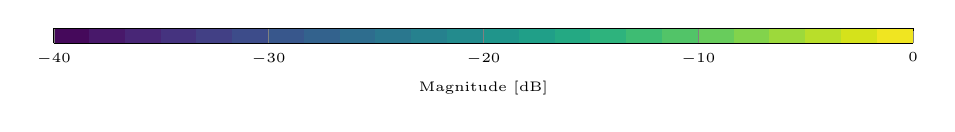
\begin{tikzpicture}
  \begin{axis}[
    hide axis,
    scale only axis,
    width=0.78\linewidth,
    height=0pt,
    colormap/viridis,
    point meta min=-40,
    point meta max=0,
    colorbar,
    colorbar horizontal,
    colorbar sampled,
    colorbar style={
      width=0.9\linewidth,
      height=1.9mm,
      at={(0.5,0)}, anchor=south,
      xtick={-40,-30,-20,-10,0},
      xticklabel style={font=\tiny},
      xlabel={Magnitude [dB]},
      xlabel style={font=\tiny, yshift=1pt},
      scaled ticks=false,
    },
  ]
    \addplot [draw=none] coordinates {(0,0)};
  \end{axis}
\end{tikzpicture}

\vspace{0.3cm}

{\color{frameblue}
The learned spectral responses provide adaptive EEG representations before directed connectivity modeling with Takens-based kernel Transfer Entropy
}

\end{frame}
%--------------------------------------------

% \begin{frame}{Results Proposal 2: Tuned Hyperparameters}

% \centering

% Best TEKTE-Net configurations selected by Bayesian optimization

% \vspace{0.12cm}

% \tiny
% \renewcommand{\arraystretch}{0.88}
% \setlength{\tabcolsep}{4pt}

% \resizebox{0.5\textwidth}{!}{
% \begin{tabular}{lcccccc}
% \toprule
% \textbf{Group} & \textbf{Subject} & \textbf{$D$} & \textbf{$D'$} & \textbf{$\tau$} & \textbf{$\mu$} & \textbf{$K$} \\
% \midrule
% \multirow{3}{*}{High} 
% & 9 & 3 & 2 & 1 & 5 & 125\\
% & 8 & 1 & 3 & 1 & 3 & 123\\
% & 3 & 3 & 8 & 2 & 0 & 63\\
% \midrule
% \multirow{3}{*}{Mid} 
% & 7 & 5 & 1 & 1 & 3 & 81\\
% & 1 & 1 & 1 & 1 & 8 & 91\\
% & 5 & 6 & 6 & 5 & 9 & 121\\
% \midrule
% \multirow{3}{*}{Low} 
% & 6 & 5 & 5 & 4 & 10 & 99\\
% & 4 & 4 & 3 & 2 & 8 & 51\\
% & 2 & 10 & 2 & 1 & 0 & 57\\
% \bottomrule
% \end{tabular}
% }

% \vfill

% {\color{frameblue}\small
% The selected configurations show subject-specific optimal dynamics, reflecting the variability of MI-EEG decoding across users
% }

% \end{frame}
% %----------------------------------------------------
%----------------------------------------------------
\begin{frame}{Results Proposal 2: Official Test Performance}

\centering
\large
Per-subject validation and official test metrics

\vspace{0.15cm}

\scriptsize
\renewcommand{\arraystretch}{1.12}
\resizebox{0.7\textwidth}{!}{
\begin{tabular}{crrrrr}
\toprule
\textbf{Subject} & \textbf{Val. Acc. (\%)} & \textbf{Acc. (\%)} & \textbf{F1 (\%)} & \textbf{Sens. (\%)} & \textbf{Spec. (\%)}\\
\midrule
9 & $99.1 \pm 1.9$  & $90.0$ & $90.1$ & $90.8$ & $89.2$\\
8 & $98.5 \pm 2.0$  & $92.5$ & $92.8$ & $94.1$ & $90.9$\\
3 & $94.2 \pm 6.0$  & $93.4$ & $93.9$ & $98.6$ & $88.1$\\
7 & $91.7 \pm 6.9$  & $77.1$ & $78.7$ & $85.5$ & $69.0$\\
1 & $89.9 \pm 8.3$  & $85.1$ & $85.3$ & $87.1$ & $83.1$\\
5 & $88.4 \pm 5.1$  & $74.8$ & $75.0$ & $78.5$ & $71.4$\\
6 & $72.6 \pm 8.4$  & $73.1$ & $71.3$ & $65.5$ & $81.1$\\
4 & $72.3 \pm 13.7$ & $75.0$ & $74.8$ & $75.4$ & $74.6$\\
2 & $67.7 \pm 8.4$  & $59.9$ & $66.7$ & $80.3$ & $39.4$\\
\midrule
\textbf{Avg} & $\mathbf{86.0 \pm 2.5}$ & $\mathbf{80.1}$ & $\mathbf{81.0}$ & $\mathbf{84.0}$ & $\mathbf{76.3}$\\
\bottomrule
\end{tabular}
}

\vfill

{\color{frameblue}\small
TEKTE-Net achieved $80.1\%$ average test accuracy and $81.0\%$ F1-score, with high-performing subjects reaching above $90\%$ accuracy
}
\end{frame}
%----------------------------------------------------
% \subsection{Attention-based Connectivity Learning}
\begin{frame}{Proposal 3: Attention-based Conectivity Learning (Aim 3)}

\begin{figure}
    \centering
    \includegraphics[width=0.7\linewidth]{figures/TEFORMER.pdf}
    \label{fig:placeholder}
\end{figure}


{\centering \textcolor{frameblue}{The proposed framework combines self-attention mechanisms with \\ Transfer Entropy to model contextual EEG dynamics and extract interpretable \\directed connectivity patterns \cite{vafaei2025transformers}} \par}

\end{frame}

%--------------------------------------------
\begin{frame}{Proposal 3:Transformer-based Temporal Attention}
    \begin{columns}
        \column{0.55\textwidth}
            \centering
            \resizebox{1\linewidth}{!}{%
                \includegraphics{figures/tgarnet_transformer}
            }
        \column{0.45\textwidth}
            \begin{enumerate}
                \item \textbf{Tokenization:} each time step 
                      treated as a $C$-dimensional token.
                \item \textbf{Multi-head self-attention 
                      ($H=2$):}
                \[
                    \mathrm{head}_h = \mathrm{softmax}
                    \!\left(\frac{\mathbf{Q}_h\mathbf{K}_h^\top}
                    {\sqrt{C_h}}\right)\mathbf{V}_h
                \]
            \end{enumerate}
    \end{columns}

\vspace{1.55cm}

{\centering 
\textcolor{frameblue}{ 
The proposed approach investigates how temporal attention can complement \\ directed connectivity modeling, enabling the extraction of context-aware and interpretable \\ EEG interaction patterns \cite{zhou2025discovery}
} 
\par}
\end{frame}
%--------------------------------------------

\begin{frame}{Experimental Set-up TEKTE-Net: ADHD/Control EEG}

\setlength{\leftmargini}{1.4em}
\setlength{\fboxsep}{1.2pt}

\vspace{0.35cm}

%==================================================
% 1. TRAINING AND VALIDATION
%==================================================
\noindent
\colorbox{frameblue}{\textcolor{white}{\textbf{\scriptsize 1}}}
\hspace{0.12cm}
\textbf{\normalsize Training and Validation:}

\vspace{0.04cm}

\begin{itemize}\itemsep2pt
    \item Validation: StratifiedGroupKFold with $5$ folds, preserving class balance and grouping by subject
    \item Training: Adam optimizer, batch size $=16$, up to $100$ epochs
    \item Loss function: binary cross-entropy with logits
    \item Regularization: early stopping and best-model checkpointing based on validation loss
\end{itemize}

\vspace{0.18cm}

%==================================================
% 2. HYPERPARAMETER SEARCH AND EVALUATION
%==================================================
\noindent
\colorbox{frameblue}{\textcolor{white}{\textbf{\scriptsize 2}}}
\hspace{0.12cm}
\textbf{\normalsize Optimization and Evaluation:}

\vspace{0.04cm}

\begin{itemize}\itemsep2pt
    \item Hyperparameter search: Optuna with $20$ trials
    \item Tuned: Transformer size, TEKTE parameters $K$, $\tau$, $\mu$, $D$, and $D'$, dropout, and learning rate.
\end{itemize}

\end{frame}
%--------------------------------------------
\begin{frame}{ Preliminar Results Proposal 3: Official Test Performance}

\centering Performance comparison across models using the official test set Metrics are \\ reported as mean $\pm$ standard deviation in percentage

\begin{table}
\centering
% \scriptsize
\label{tab:model_comparison_results}
\resizebox{\textwidth}{!}{%
\begin{tabular}{lcccc}
\hline
\textbf{Model} & \textbf{Accuracy (\%)} & \textbf{Recall (\%)} & \textbf{Precision (\%)} & \textbf{AUC (\%)} \\
\hline

T-GARNet & $77.4 \pm 6.8$ & $85.5 \pm 10.8$ & $76.9 \pm 7.4$ & $84.1 \pm 7.8$ \\ EEGNet & $81.5 \pm 6.9$ & $83.5 \pm 12.0$ & $84.3 \pm 8.6$ & $88.8 \pm 8.6$ \\ ShallowConvNet & $\mathbf{83.7 \pm 11.1}$ & $82.5 \pm 18.7$ & $\mathbf{86.9 \pm 9.1}$ & $\mathbf{90.3 \pm 10.3}$ \\ Multi-Stream Transformer & $58.6 \pm 3.4$ & $\mathbf{86.5 \pm 9.4}$ & $58.7 \pm 2.3$ & $58.7 \pm 6.8$ \\ IM--CBGT & $66.1 \pm 4.5$ & $74.4 \pm 11.9$ & $68.2 \pm 4.6$ & $71.2 \pm 6.7$ \\ \textbf{TE-Former (Ours)} & $80.7 \pm 5.1$ & $84.0 \pm 9.6$ & $82.2 \pm 6.8$ & $87.8 \pm 5.7$ \\

\hline
\end{tabular}%
}
\end{table}

\vspace{-0.15cm}
\begin{center}
{\color{frameblue}
Preliminary results suggest that the proposed model achieves competitive and balanced performance across metrics, while showing reduced variability compared with several baseline architectures}
\end{center}

\end{frame}
%-----------------------------


\section{Conclusions}

\begin{frame}{Conclusions}

\begin{itemize}

\item \textbf{Connectivity-driven EEG imaging} provided a more robust representation of MI-EEG signals by transforming \textbf{inter-channel relationships into topographic maps}. In the GIGA MI dataset, EEG-GCIRNet improved subject-wise performance across low-, mid-, and high-performing subjects, supporting the usefulness of \textbf{Gaussian functional connectivity} and \textbf{latent-space regularization} to mitigate noisy and spatially mixed EEG patterns. \textbf{(Obj. 1)}

\vspace{0.25cm}

\item \textbf{TEKTE-Net} enabled the modeling of \textbf{nonlinear, delayed, and directed EEG dependencies} through Takens state-space reconstruction and kernel Transfer Entropy. In BCI Competition IV-2a, the model achieved competitive subject-wise decoding performance and produced \textbf{interpretable directed connectivity patterns} associated with left- and right-hand motor imagery. \textbf{(Obj. 2)}

\end{itemize}
\end{frame}
%----------------------------------------------------
\section{Future Work}
\begin{frame}{Future Work}

\begin{itemize}

\item Integrate \textbf{attention mechanisms} into connectivity-aware deep learning models to adaptively weight \textbf{task-relevant EEG interactions}.

\item Extend the Takens-based kernel Transfer Entropy framework toward \textbf{connectivity transformers} for modeling \textbf{spatiotemporal and directed dependencies}.

\item Improve \textbf{subject-independent generalization} by reducing the impact of \textbf{inter- and intra-subject variability} and domain shift.

\item Preserve \textbf{neurophysiological interpretability} by identifying stable and meaningful \textbf{connectivity patterns} across subjects and tasks.

\end{itemize}

\end{frame}

% %----------------------------------------------------

%----------------------------------------------------
\begin{frame}{Academic products}
% \scriptsize
\begin{itemize}
  \item \textbf{Publications}
  \begin{itemize}\itemsep3pt

    \item \textbf{Conference Paper:} Gomez-Rivera, A.; Cardona-Álvarez, Y.; Gomez-Morales, O. W.; Alvarez-Meza, A. M.; Castellanos-Domínguez, G.
    \emph{BCI-based real-time processing for implementing deep learning frameworks using MI paradigms.}
    Journal of Applied Research and Technology, Oct 30, 2024.\\
    \href{https://doi.org/10.22201/icat.24486736e.2024.22.5.2392}{DOI}

    \item \textbf{Journal Paper (Q1):} Gomez-Rivera, A.; Collazos-Huertas, D. F.; Cárdenas-Peña, D.; Álvarez-Meza, A. M.; Castellanos-Domínguez, G.
    \emph{A Gaussian Connectivity-Driven EEG Imaging for Deep Learning-Based Motor Imagery Classification.}
    Sensors, 2026, 26, 227.\\
    \href{https://doi.org/10.3390/s26010227}{DOI}

    \item \textbf{Journal Paper (Q1):} Gomez-Rivera, A.; Álvarez-Meza, A. M.; Cárdenas-Peña, D.; Orozco-Gutierrez, A.
    \emph{Takens-Based Kernel TE Connectivity Network for Motor Imagery Classification.}
    Sensors, 2025, 25, 7067.\\
    \href{https://doi.org/10.3390/s25227067}{DOI}

  \end{itemize}
\end{itemize}
\end{frame}

%----------------------------------------------------
\begin{frame}{Academic products}
% \scriptsize
\begin{itemize}

  \item \textbf{Publications}
  \begin{itemize}\itemsep3pt

    \item \textbf{Journal Paper (Q1, accepted for publication):} Pastrana-Cortés, J. D.; Gomez-Rivera, A.; Álvarez-Meza, A. M.; Gil-Gonzalez, J.; Cárdenas-Peña, D.
    \emph{Temporal Attention and Convolutional Tokenization for Interpretable ADHD Classification from EEG.}
    Accepted for publication, 2026.\\
    \href{https://www.preprints.org/frontend/manuscript/8cf77def865d68c2bf3c9887e397e670/download_pub}
    {Preprint available at Preprints.org}

  \end{itemize}

  \vspace{0.12cm}

  \item \textbf{Software and repositories}
  \begin{itemize}\itemsep3pt

    \item \textbf{EEG-GCIRNet}: Open-source implementation of the Gaussian connectivity-driven EEG imaging framework proposed in this thesis.\\
    \href{https://github.com/alegomezri/EEG-GCIRNet}{GitHub repository}

    \item \textbf{TEKTE-Net}: Open-source implementation of the Takens-based kernel transfer entropy connectivity network for effective connectivity modeling.\\
    \href{https://github.com/alegomezri/TEKTE-Net}{GitHub repository}

  \end{itemize}

\end{itemize}
\end{frame}

%----------------------------------------------------
\begin{frame}{Academic products}
% \scriptsize
\begin{itemize}

  \item \textbf{Patents and Technology Transfer}
  \begin{itemize}\itemsep3pt
    \item \textbf{NC2022/0007405 -- Método y sistema para la sincronización de marcadores asociados a sistemas de interfaz cerebro--computador.}\\
    Patent application filed before the Superintendence of Industry and Commerce (SIC), Colombia, on May 28, 2022.\\
    \textit{Current status:} Patentability examination.
  \end{itemize}

  \vspace{0.12cm}

  \item \textbf{Planned international research stay}
  \begin{itemize}\itemsep3pt
    \item A research stay is planned at the 
    \textbf{Instituto Argentino de Matemática ``Alberto P. Calderón'' 
    (IAM-CONICET)}, Buenos Aires, Argentina.
    
    \item The stay will be carried out in collaboration with 
    \textbf{Dra. María Paula Bonomini}, focusing on the development of 
    attention-based connectivity learning methods for EEG analysis.
  \end{itemize}

  \vspace{0.12cm}

  \item \textbf{Manuscript in preparation}
  \begin{itemize}\itemsep3pt
    \item A collaborative manuscript is currently under preparation with 
    IAM-CONICET, focused on the current work:
    
    \emph{Attention-based Connectivity Learning for Interpretable EEG Decoding.}
    
  \end{itemize}

\end{itemize}
\end{frame}

%--------------------------------------------

\begin{frame}{Implementation Schedule}
\centering
\scriptsize
\setlength{\tabcolsep}{7pt}
\renewcommand{\arraystretch}{0.95}

\begin{tabular*}{\textwidth}{@{\extracolsep{\fill}} l*{11}{c}}
\toprule
\textbf{Months} &
\multicolumn{2}{c}{\textbf{Objective 1}} &
\multicolumn{2}{c}{\textbf{Objective 2}} &
\multicolumn{2}{c}{\textbf{Objective 3}} &
\multicolumn{3}{c}{\textbf{Future Work}} &
\multicolumn{2}{c}{\textbf{Dissemination}} \\
\cmidrule(lr){2-3}\cmidrule(lr){4-5}\cmidrule(lr){6-7}\cmidrule(lr){8-10}\cmidrule(lr){11-12}
& 1a & 1b & 2a & 2b & 3a & 3b & FW1 & FW2 & FW3 & Papers & Thesis \\
\midrule

\rowcolor{completed}  1--3   & \cmark &        & \cmark &        &        &        &        &        &        &        &        \\
\rowcolor{completed}  4--6   & \cmark & \cmark & \cmark & \cmark &        &        &        &        &        &        &        \\
\rowcolor{completed}  7--9   &        & \cmark &        & \cmark &        &        &        &        &        & \cmark &        \\
\rowcolor{completed} 10--12  &        & \cmark &        & \cmark &        &        &        &        &        &        &        \\
\rowcolor{completed} 13--15  &        & \cmark &        & \cmark &        &        &        &        &        & \cmark &        \\
\rowcolor{completed} 16--18  &        & \cmark &        & \cmark &        &        &        &        &        & \cmark &        \\
\midrule

19--21  &        &        &        &        & \cmark &        &        &        &        &        &        \\
22--24  &        &        &        &        & \cmark & \cmark & \cmark &        &        &        &        \\
25--27  &        &        &        &        &        & \cmark & \cmark & \cmark &        &        & \cellcolor{writing}\wmark \\
28--30  &        &        &        &        &        & \cmark &        & \cmark & \cmark &        & \cellcolor{writing}\cmark \\
31--33  &        &        &        &        &        &        &        &        & \cmark & \cmark & \cellcolor{writing}\cmark \\
34--36  &        &        &        &        &        &        &        &        &        & \cellcolor{paperblue}\cmark & \cellcolor{writing}\cmark \\
\bottomrule
\end{tabular*}

\vspace{0.6em}
\tiny
\textbf{36-month implementation schedule} (current progress: \textbf{Month 18}).\\[0.3ex]
\textbf{Legend:} \cmark = completed/planned milestone \hspace{1em}
\wmark\ / shaded orange = thesis-writing phase\\[0.4ex]
\textbf{Task codes:}
1a/2a – theoretical formulation and methodological definition; 1b/2b – implementation, experimentation, and validation;\\
3a – inter- and intra-subject variability analysis and mitigation; 3b – interpretable representation analysis and validation;\\
FW1 – subject-independent generalization and robustness to variability; FW2 – advanced interpretability and representation analysis; FW3 – evaluation in broader and applied BCI scenarios.
\end{frame}
%--------------------------------------------

\begin{frame}{Acknowledgments}


   \textit{I recognize that this research would not have been possible without the support given by the project
    “Alianza científica con enfoque comunitario para mitigar brechas de atención y manejo de trastornos
    mentales y epilepsia en Colombia (\textbf{ACEMATE})-91908” funded by Minciencias.}


\begin{center}
	{\Huge{\textbf{\textcolor{frameblue}{Thank you!}}}}\\
	\vspace{0.2cm}
    \textbf{Contact:}\\
    \vspace{0.2cm}
	 Yessica Alejandra Gomez Rivera\\ {\scriptsize{yeagomezri@unal.edu.co}}\\

\end{center}    
    
\end{frame}

%--------------------------------------------
\begin{frame}[allowframebreaks]%,noframenumbering]
\frametitle{References}
{\tiny 
\bibliographystyle{apalike}
\bibliography{references}
}
\end{frame}
\end{document}


















